\documentclass[a5paper,12pt,twoside]{book} % Book style options
\usepackage[backgroundcolor=white,  %
			bordercolor=black,      %
			linecolor=black,        %
			textsize=tiny,          %
			textwidth=1.8cm,        %
			]{todonotes}            % To-Do notes package (to be removed)
\usepackage{graphicx}               % For plotting figures
\usepackage[skip=0.2cm]{caption}    % Change spacing from caption
\usepackage{CJKutf8}                % To use Chinese, Japanese and Korean characters
\newcounter{joseki}                 % Set a counter for the number of josekis used in the contents
\usepackage[english]{babel}         % Load English language for dictionary
\usepackage[hidelinks]{hyperref}    % Used for cross-references and hyperlinks           
%\usepackage{makeidx}                % Used to make index
%\makeindex                          % Make index command
%\usepackage[totoc]{idxlayout}       % Add index to Table of Contents
\usepackage{igo}	                % Load IGO package for plotting goban diagrams
\usepackage[margin=2.2cm]{geometry} % Change the geometry of the page
\usepackage{wrapfig}
\usepackage{titlesec}




\AtBeginDocument{%
\renewcommand{\figurename}{Diagram}  % Change name of figure label
}

% Define paths for gobans and images
\makeatletter
\def\input@path{{gobans/}}
\makeatother
\graphicspath{{images/}}

%%%%% latex -interaction=nonstopmode %.tex|latex -interaction=nonstopmode %.tex|makeindex %.idx|makeglossaries %|latex -interaction=nonstopmode %.tex|latex -interaction=nonstopmode %.tex|dvips -Pdownload35 -o %.ps %.dvi|ps2pdf %.ps|"C:/Program Files (x86)/FOXIT SOFTWARE/FOXIT READER/FoxitReader.exe" %.pdf

% Commands for diagram cross-refferences
\newcommand{\dref}[1]{Diagram \ref{#1}} 
\newcommand{\drefs}[1]{Dia. \ref{#1}} 

% Manually add items to Table of Contents
\newcommand{\addstufftotoc}[2][toc]{%
  \addtocontents{#1}{#2}}
  
% Title page options
\title{\textit{An introductory guide to}\\\vspace{0.5cm} {\Huge Joseki}}
\author{}
\date{ }

\begin{document}
% Insert OSR logo in the title-page
\vbox{
\centering
\vspace{1.5cm}

\includegraphics[width=0.8\textwidth]{OSR.eps}
\\\vspace{2cm}
\large{presents}
\\\vspace{-1.5cm}
\maketitle
}
\clearpage{\thispagestyle{empty}\cleardoublepage}

\frontmatter
\listoftodos

\chapter{Glossary}
%\addcontentsline{toc}{chapter}{Glossary}

Go, like chess, has international popularity. Originating in China, it also has a long and rich history in Japan and Korea. Naturally, then, there are many terms describing moves, shapes, sequences, and other parts of the game that have a different name in Chinese, Japanese, and Korean. When Go was introduced to Europe and America in the late-19th and early-20th centuries, it was with the aid of Japanese pioneers and the available study material largely came from Japanese sources. In this way, many Japanese terms gained currency in the West. The English-speaking Go community, though, have also developed a variety of their own words.\\
\indent Material written about Go in English in the last decade has typically employed a mix of Japanese and English terms, with a few exceptions (such as Korean \textit{haengma}, meaning roughly `movement of the stones'). In this book, we have followed this convention and generally tried to use the most commonly-used name for each concept. The glossary below provides a list of terms used in the book with their definitions, listed when possible with both their English and Japanese aliases.\\

\noindent Key: n. = noun, v. = verb, adj. = adjective\\

\noindent \textit{aji} (n.): The potential for a player to play a sequence or sequences in a local area, in the vicinity of the opponent's group. To actually play the sequence is to use or exploit the \textit{aji}. If the possible sequence would damage a group, the \textit{aji­} is called \textit{bad aji}.\\

\noindent \textit{atari} (n., v.): To \textit{atari} a group is to reduce it to having only one liberty, allowing it to be captured unless the opponent defends the group. As a noun, an \textit{atari} is a move that makes an \textit{atari}. Some Western players announce \textit{atari} in their games but this is not necessary and is in fact often frowned upon.\\

\noindent \textit{boshi} / cap (n., v.): A move made one empty space above a stone with the intention of preventing it from rising higher on the board, a tactic used in reduction and attack. Or, a 4-4 point played against a 3-3, again with the intention to constraining development. To cap is to play such a move.\\

\noindent \textit{fuseki} / opening (n.): The first moves of a game, in which \textit{joseki} are played and developmental points are occupied. The length of the opening is usually considered to be contextual to the progression of the game, and dependent on the focus of the observer, but a common number cited is thirty moves. The term \textit{fuseki} can also apply more narrowly to opening theory.\\

\noindent \textit{gote} (adj.): A move that does not require a response, often but not always a forced move. A player who makes a \textit{gote} move can be said to have taken \textit{gote} or been put in \textit{gote}. In this sense, it is the opposite of sente. \textit{Gote} is an alternative name for White, as White moves second.\\

\noindent \textit{hane} (n., v.): A diagonal move that `turns against' an opponent's stone.\\

\noindent \textit{joseki} (n.): A sequence of moves in and around a corner judged by professionals to constitute the best local play (in a common whole-board context). More loosely, a \textit{joseki} can be a sequence once considered optimal but now superseded. A \textit{joseki} move is a move that follows a \textit{joseki} sequence.\\

\noindent \textit{keima} / knight’s move (n., v.): A move two spaces forward and one space left or right, like the jump made by the knight piece in chess. The \textit{ogeima} is a similar but larger move. To \textit{keima} is to play a \textit{keima}.\\

\noindent \textit{kosumi} / diagonal (n., v.): A diagonal move that does not leave empty space. To \textit{kosumi} is to make such a move.\\

\noindent \textit{moyo} / framework (n.): A coordination of stones that surrounds a large area of the board on the side or in the centre. A \textit{moyo} is usually not entirely solid territory and is open to reduction or invasion. The term \textit{framework} can also have a broader meaning, referring to the coordination of one player's stones more generally.\\

\noindent \textit{ogeima} / Large knight's move (n., v.): A move three spaces forward and one space left or right. To \textit{ogeima} is to play an \textit{ogeima}.\\

\noindent \textit{sente} (n., adj.): The initiative, i.e. the opportunity to play an unforced move. The phrases to have, take, and keep \textit{sente} all refer to this sense. A \textit{sente} move is a move that demands a response and in this sense is the opposite of \textit{gote}. \textit{Sente} is an alternative name for Black, as Black moves first.\\

\noindent \textit{shimari} / enclosure (n., v.): A shape, made out of two or three stones, used to surround a corner. To \textit{shimari} is to make a \textit{shimari}.\\

\noindent \textit{tenuki}  (n., v.): To play away from a local position, moving to another part of the board. A \textit{tenuki} is a move that does this.

\clearpage

\addcontentsline{toc}{chapter}{Contents}
\tableofcontents


\chapter{Preface}
%\addcontentsline{toc}{chapter}{Preface}
This guide aims to be a collection of simple, solid \textit{joseki} for practical use. It is aimed at a player of 10 \textit{kyu} level or weaker, and sets out to provide the reader with a repertoire of sequences that they can be confident to play in and around the corner.\\

First of all, what do we mean by \textit{joseki}? \textit{Joseki} (\begin{CJK}{UTF8}{min}定石\end{CJK}) is a Japanese word, literally meaning `settled stones'. In its strictest real usage, it refers to a sequence of moves by both players in and around a corner, that are judged by professionals to be the best local plays discovered. So then, as professionals discover better local moves, only the best and most recent sequences are really \textit{joseki}. However, in broader use of the term, \textit{joseki} can refer to any sequence that was ever considered to be optimal by professionals, even if they may have been discarded over the course of time. None of the sequences put forward by this guide will be on the cutting edge of theory, nor will they all be thought by professionals to be best for both players. They are sequences that are `good'  – they will function as sound, strong building blocks on which to build your positions. The correct choice of \textit{joseki} varies according to the whole-board position.\\

The \textit{joseki} in this guide are formatted in diagrams of the traditional Oriental kind. Numbers on the stones show the order of moves, rather than a series of coordinates as in chess notation. Where alternate moves are discussed, they are indexed by a letter placed on their position on the board. The guide is formatted into five sections, based on the five orthodox opening moves: the 3-3 (\textit{san-san}), 3-4 (\textit{komoku}), 5-3 (\textit{mokuhazushi}), 4-4 (\textit{hoshi}) and 5-4 (\textit{takamoku}). In practice, the 3-4 and 4-4 points are played much more frequently than the others listed. Equally, there are other moves that are played rarely but are not included, such as the 4-6 (\textit{ootakamoku}) and 5-5 (\textit{gonogo}) points.\\

\mainmatter

\chapter{The 3-3 (\textit{san-san}) \label{sec:3-3}}
The 3-3 is a modern move, pioneered in the experimental \textit{shin} \textit{joseki} (new openings) period of the 1930s and 1940s. Its advantages are to take solid territory, to settle the corner in a single move (that is to say, an approach by the opponent will not be as large as against a 3-4), and to establish a definitely living group. The last point can be relevant in cross-openings, in which each player holds two corners diagonally opposite one another, leaving groups potentially vulnerable to attack. The disadvantages of the 3-3, like its advantages, lie in its low position on the board: it is hard to develop a large side territory from, and the opponent can approach it from above or press it down from the centre.\\

\section{The cap}
The simplest 3-3 \textit{joseki} is the cap, shown in \dref{the-cap:1}:

\begin{figure}[!htbp]
\begin{center}
\smallgoban
\cleargoban
\black{c3}
\white[1]{d4}
\gobansymbol{c4}{A}
\gobansymbol{d3}{B}
\rotategoban
\mirrorgoban
\showgoban
\end{center} 
\vspace{-0.6cm}\caption{The cap approach}
\label{the-cap:1}
\end{figure}

White plays the 4-4 point, leaving Black with two local options: to push at A or at B. In this diagram, the two options appear the same. But in a realistic whole-board position, it is probable that the positions on each side of the board will be different, so it can be important to choose the right direction from which to push\footnote{Add a small footnote to say how to choose?}.\\

Black can also consider \textit{tenuki}'ing, which leaves white the option of continuing locally, again at A or B. This transposes to a 3-3 invasion beneath a 4-4, so we will deal with it in more detail in Chapter \ref{sec:4-4}. The capping play{\large\whitestone[1]} is typically considered to be smaller than an approach to or invasion of another of the normal corner-occupying moves. This is for two reasons: i) Black does not stand to lose territory from being capped; and ii) Black will not be easily able to develop on a large scale from his 3-3 stone.\\

\begin{figure}[!htbp]
\begin{center}
\smallgoban
\cleargoban
\black{c3}
\white[1]{d4,d3,e4}
\gobansymbol{c4}{A}
\rotategoban
\mirrorgoban
\showgoban
\end{center}
 
\vspace{-0.6cm}\caption{The cap developing}
\label{3-3:2}
\end{figure}

Continuing from \dref{the-cap:1}, after Black pushes with{\large\blackstone[2]} in \dref{3-3:2}, White must play{\large\whitestone[3]}. If she blocks at A, Black will play{\large\blackstone[3]} himself. Black will have the `\textit{hane} on the head of two stones', a good shape, and White's shape will be weak.\\

\begin{figure}[!htbp]
\begin{center}
\smallgoban
\cleargoban
\black{c3}
\white[1]{d4,d3,e4,b5,d7,f2,h4}
\gobansymbol{c4}{A}
\gobansymbol{e3}{B}
\rotategoban
\mirrorgoban
\hyperref[3-3:the-cap]{\showgoban}
\end{center}
\vspace{-0.6cm}\caption{The cap}
\label{3-3:the-cap}
\end{figure}

The \textit{joseki} in \dref{3-3:the-cap} is a common capping \textit{joseki}. Black uses the \textit{keima} to secure access to the sides of the board; if he omitted these moves then White would have effective plays at A and B, sealing Black into the corner. Note that White's jumps are two spaces, not one space. If they were one space, they would be too close to make efficient use of White's two-stone wall{\large\whitestone[1]} \&{\large\whitestone[3]}. In the settled position, White has taken influence towards the centre and Black has taken the corner. After the attack from White, Black has \textit{sente}.\\

White should play this when she wants more influence. However, she must be careful not to play it too early. That is because depending on the course of the opening, White's stones can become a weak group as they have no base on the side or in the corner. It is often better to wait until some other \textit{joseki} and opening moves have been played, and judging by the whole-board position, one can decide if it is in their favour committing to take influence like this.\\

\begin{figure}[!htbp]
\begin{center}
\smallgoban
\cleargoban
\black{c3}
\white[1]{d4,d3,e4,b5,e3,d6,j3}
\gobansymbol{e6}{A}
\rotategoban
\mirrorgoban
\hyperref[3-3:the-cap-full]{\showgoban}
\end{center}
\vspace{-0.6cm}\caption{The cap alternative response}
\label{3-3:the-cap-full}
\end{figure}

Though not as common as the first capping sequence shown, White will sometimes turn at{\large\whitestone[5]} if she wishes to focus on the right side. In this case, Black can play the \textit{keima}{\large\blackstone[6]} to raise his position on the top side. He can do this because White omitted to make the two-space extension along that side which would otherwise have pressed Black down, as was shown in \dref{3-3:the-cap}. Before or instead of extending at{\large\whitestone[7]}, White can also consider attaching at A to attempt to gain a bit more thickness on the outside. But because that introduces more length and complication to the sequence, it will not be covered in here.\\

\section{The \textit{ogeima} approach}

White may approach with an \textit{ogeima} rather than cap, like in the diagram below.

\begin{figure}[!htbp]
\begin{center}
\smallgoban
\cleargoban
\black{c3}
\white[1]{d6,f3,d9}
\gobansymbol{f4}{A}
\mirrorgoban
\rotategoban
\hyperref[3-3:ogeima]{\showgoban}
\end{center} 
\vspace{-0.6cm}\caption{The ogeima approach}
\label{3-3:ogeima}
\end{figure}

In this case, it is advisable for Black to make a two-space base to provide stability for his group; and for White to settle her stones in a similar fashion. Black can also choose to play{\large\blackstone[2]} at A for a higher position, if the centre is important. Note, though, that White's group (being on the fourth line) is vulnerable to having its base stolen from beneath, especially if it is surrounded by hostile groups. For this reason, it is recommended that White only plays this way when she has strength in the top left for the configuration in \dref{3-3:ogeima}.\\
\addstufftotoc{\nobreak\smallskip\protect\begin{minipage}[b][][b]{.5\textwidth}
\centering
\begin{center}
\smallgoban
\cleargoban
\black{c3}
\white[1]{d4,d3,e4,b5,d7,f2,h4}
\rotategoban
\mirrorgoban
\hyperref[3-3:the-cap]{\showgoban}
\end{center}
\stepcounter{joseki}
\vspace{-0.6cm} \arabic{joseki}. The cap (pg. \pageref{3-3:the-cap})
\end{minipage}%
\begin{minipage}[b][][b]{0.5\textwidth}
\centering
\begin{center}
\smallgoban
\cleargoban
\black{c3}
\white[1]{d6,f3,d9}
\mirrorgoban
\rotategoban
\hyperref[3-3:ogeima]{\showgoban}
\end{center}
\stepcounter{joseki}
\vspace{-0.6cm} \arabic{joseki}. The ogeima (pg. \pageref{3-3:ogeima})
\end{minipage}\par}

\chapter{The 3-4 (\textit{komoku}) \label{sec:3-4}}

Before the \textit{shin fuseki} period in the early 20th century, the 3-4 point was the move of choice by most professional players to occupy the corner. Its advantage was, and is, in presenting a compromise between territory and influence. It is neither as low as the 3-3 point (Ch.~\ref{sec:3-3}), losing control of the centre, or as high as the 4-4 (Ch.~\ref{sec:4-4}) or 5-4 (Ch.~\ref{sec:5-4}) points which only a weak grasp on the corner. As a result of its frequent appearance, there are many 3-4 \textit{joseki}s and some of them have the potential to become very complex. The three most complicated \textit{joseki} - the \textit{taisha} (`great slant'), the avalanche or \textit{nadare}, and the magic sword\todo{Clarify which ones we are covering.}; all develop from the 3-4. But that doesn't mean that a sufficient choice of simple and solid 3-4 \textit{joseki} is not available.\\

When playing against the 3-4 point, White can choose from four different approaches, A to D, as shown in \dref{3-4:approach}.\todo{Capital or maybe use lower case letters?} \todo{Example with lower-case letters.}\\

\begin{figure}[!htbp]
\begin{center}
\smallgoban
\cleargoban
\black{d3}
\gobansymbol{c5}{a}
\gobansymbol{d5}{b}
\gobansymbol{c6}{c}
\gobansymbol{d6}{d}
\mirrorgoban
\rotategoban
\showgoban
\end{center} 
\vspace{-0.6cm}\caption{The 3-4 approach options}
\label{3-4:approach}
\end{figure}


Of these, A (the low approach) and B (the high approach) are most popular. Often, the reason for playing C or D is to avoid being pincered; or to avoid being kicked and attacked in an area where Black is strong.\\

\section{The far approach (C)}
\todo{Shall we order them A to D as they are presented?}

\begin{figure}[!htbp]
\begin{center}
\smallgoban
\cleargoban
\black{d3}
\white[1]{c6,c4,c9,g3}
\gobansymbol{d5}{a}
\gobansymbol{f3}{b}
\mirrorgoban
\rotategoban
\hyperref[3-4:far-approach]{\showgoban}
\end{center} 
\vspace{-0.6cm}\caption{The far approach}
\label{3-4:far-approach}
\end{figure}

If White approaches with C, the far approach, then this is the simplest variation. Black defends the corner, White settles her group with a two-space base, and Black extends onto the side. Black may also play{\large\blackstone[2]} at A, shoulder-hitting{\large\whitestone[1]}. That \textit{joseki} often appears in the early stages of the \textit{Kobayashi} opening. The reason why Black uses{\large\blackstone[4]} to extend along the side rather than making a \textit{tenuki}, is because if White gets to extend to{\large\whitestone[4]} or even B then the corner would become too cramped.\\

\section{The far high approach (D)}

\begin{figure}[!htbp]
\begin{center}
\smallgoban
\cleargoban
\black{d3}
\white[1]{d6,c5,c6,d5,e6}
\mirrorgoban
\rotategoban
\hyperref[3-4:far-high-approach]{\showgoban}
\end{center}
\vspace{-0.6cm}\caption{The far high approach}
\label{3-4:far-high-approach}
\end{figure}

If White makes the far high approach as in \dref{3-4:far-high-approach}, Black can play{\large\blackstone[2]} to defend the corner. This \textit{joseki} is locally bad for White, so it is not recommended unless White already has development on the top side that can be significantly enhanced by{\large\whitestone[1]},{\large\whitestone[3]} \&{\large\whitestone[5]}. Alternatively, White can push at{\large\whitestone[4]}, which will transpose into another 3-4 \textit{joseki}.\\

\addstufftotoc{\nobreak\smallskip\protect\begin{minipage}[b][][b]{.5\textwidth}
\centering
\begin{center}
\smallgoban
\cleargoban
\black{d3}
\white[1]{c6,c4,c9,g3}
\mirrorgoban
\rotategoban
\hyperref[3-4:far-approach]{\showgoban}
\end{center}
\stepcounter{joseki}
\vspace{-0.6cm} \arabic{joseki}. The far approach (pg. \pageref{3-4:far-approach})
\vspace{2pt}
\end{minipage}%
\begin{minipage}[b][][b]{0.5\textwidth}
\centering
\begin{center}
\smallgoban
\cleargoban
\black{d3}
\white[1]{d6,c5,c6,d5,e6}
\mirrorgoban
\rotategoban
\hyperref[3-4:far-high-approach]{\showgoban}
\end{center}
\stepcounter{joseki}
\vspace{-0.6cm} \arabic{joseki}. The far high approach (pg. \pageref{3-4:far-high-approach})
\vspace{2pt}
\end{minipage}\par}

\section{The high approach (B)}

The high approach is used by White to take a position that is not too low on the board, and cannot be forced upon from the centre; or sometimes to avoid being kicked. Notice that the high approach is the same thing as White \textit{tenuki}'ing from an invasion at 3-4 beneath his 5-4 corner stone. For more information, see Chapter \ref{sec:5-4}.\\

\begin{figure}[!htbp]
\begin{center}
\smallgoban
\cleargoban
\black{d3}
\white[1]{d5,c5}
\gobansymbol{f4}{A}
\gobansymbol{c6}{B}
\gobansymbol{d4}{C}
\mirrorgoban
\rotategoban
\showgoban
\end{center} 
\vspace{-0.6cm}\caption{The high approach beginning}
\label{3-4:high-approach-1}
\end{figure}

Attaching underneath with{\large\blackstone[2]} is most solid, keeping control of the corner. Black can also \textit{keima} away with A, and this can be better if the right side or centre is large; but in general it is better to play as in the diagram. White can now choose from two options, B and C.\\

\begin{figure}[!htbp]
\begin{center}
\smallgoban
\cleargoban
\black{d3}
\white[1]{d5,c5,c6,c4,d6}
\gobansymbol{b5}{A}
\gobansymbol{d7}{B}
\gobansymbol{c8}{C}
\mirrorgoban
\rotategoban
\showgoban
\end{center} 
\vspace{-0.6cm}\caption{The high approach}
\label{3-4:high-approach-2}
\end{figure}

The most usual and simple choice is to \textit{hane} at B as in \dref{3-4:high-approach-2}. Black almost always will draw back with{\large\blackstone[4]}, though there is a rare \textit{joseki} in which Black descends to A. It is not essential to learn the latter, and besides it is generally considered slightly inferior to the play in \dref{3-4:high-approach-2}. White can also play{\large\whitestone[5]} at B, making a tiger's mouth. Recently, that variation has lost favour due to a weakness in the shape at C. Playing{\large\whitestone[5]}, the full triangle, is more resilient.\\

\begin{figure}[!htbp]
\begin{center}
\smallgoban
\cleargoban
\black{d3}
\white[1]{d5,c5,c6,c4,d6,f3,c10}
\gobansymbol{e4}{A}
\gobansymbol{f4}{B}
\gobansymbol{d10}{C}
\gobansymbol{c9}{D}
\gobansymbol{c12}{E}
\gobansymbol{c8}{F}
\gobansymbol{e10}{G}
\gobansymbol{e3}{H}
\mirrorgoban
\rotategoban
\hyperref[3-4:high-approach-3]{\showgoban}
\end{center}
\vspace{-0.6cm}\caption{The high approach common settled position}
\label{3-4:high-approach-3}
\end{figure}

Following from \dref{3-4:high-approach-2}, \dref{3-4:high-approach-3} displays the most common settled position. Black must extend onto the side, or White will press down on his shape with an attachment at H. Black usually makes this extension as in the diagram, but moves at A and B are also played if Black wants a higher position. White then also extends along the side, typically to{\large\whitestone[7]}. The reason why White usually extends three spaces and not two or four is to make the most effective use of her full triangle in keeping with the proverb `extend three spaces from a two-stone wall'. White doesn't want to be inefficient, but also wants to avoid exposing weakness in her shape too easily. White often extends on the fourth line instead, at C. \\

There is an issue with this \textit{joseki}, which is the weakness at F which threatens to undermine White's base and split his stones. This defect is mainly an issue when Black has a stone at E, and so if Black plays there White will typically defend by jumping to G.\\

\subsection*{The \textit{avalanche}}
In its strict sense, the \textit{avalanche} or \textit{nadare joseki} begins when Black plays either A (the \textit{small avalanche}) or B (the \textit{large avalanche}) in \dref{3-4:avalance-1}. Both of these moves lead to challenging sequences that require memorisation, so instead it is recommended that Black plays at A. In comparison to B and C, A is considered to be a little better for White due to her solid finishing shape. But more important is that unlike Black's other options, C begins a relatively simple path that results in a solid shape. D is also played, like C, to avoid the \textit{avalanches} proper \todo{proper?} but is slightly less solid, leaving \textit{aji} in the corner.\\

It is not recommended that you play{\large\whitestone[3]} as White if you're not prepared to deal with the \textit{small} and \textit{large avalanche} variations; instead, \textit{hane} at C as discussed\footnote{Though, if you actually play{\large\whitestone[3]} and{\large\whitestone[5]} then beneath 5 \textit{kyu} level Black will almost always opt for the simple variation A.}.\\

\begin{figure}[!htbp]
\begin{center}
\smallgoban
\cleargoban
\black{d3}
\white[1]{d5,c5,d4,c4,e3}
\gobansymbol{c3}{A}
\gobansymbol{d6}{B}
\gobansymbol{c6}{C}
\gobansymbol{d2}{D}
\mirrorgoban
\rotategoban
\showgoban
\end{center} 
\vspace{-0.6cm}\caption{The avalanche development}
\label{3-4:avalance-1}
\end{figure}

You may notice that{\large\whitestone[3]} puts White into the \textit{hane} on the head of two stones shape that was condemned earlier. Sometimes, \textit{joseki} feature bad shapes due to deep overall analysis of the local position.\\

\begin{figure}[!htbp]
\begin{center}
\smallgoban
\cleargoban
\black{d3}
\white[1]{d5,c5,d4,c4,e3,c3,d6,c7,f4}
\gobansymbol{c6}{A}
\mirrorgoban
\rotategoban
\hyperref[3-4:avalance-2]{\showgoban}
\end{center} 
\vspace{-0.6cm}\caption{The small avalanche}
\label{3-4:avalance-2}
\end{figure}

\dref{3-4:avalance-2} would be the end of the sequence. White may choose to omit{\large\whitestone[9]} if she considers it more favourable to do so in the global position. Black should not omit{\large\blackstone[8]}, the jump into the top side, as a white turn at A would seal Black in.\\

\addstufftotoc{\nobreak\smallskip\protect\begin{minipage}[b][][b]{.5\textwidth}
\centering
\begin{center}
\smallgoban
\cleargoban
\black{d3}
\white[1]{d5,c5,c6,c4,d6,f3,c10}
\mirrorgoban
\rotategoban
\hyperref[3-4:high-approach-3]{\showgoban}
\end{center}
\stepcounter{joseki}
\vspace{-0.6cm} \arabic{joseki}. The high approach (pg. \pageref{3-4:high-approach-3})
\end{minipage}%
\begin{minipage}[b][][b]{0.5\textwidth}
\centering
\begin{center}
\smallgoban
\cleargoban
\black{d3}
\white[1]{d5,c5,d4,c4,e3,c3,d6,c7,f4}
\gobansymbol{c6}{A}
\mirrorgoban
\rotategoban
\hyperref[3-4:avalance-2]{\showgoban}
\end{center}
\stepcounter{joseki}
\vspace{-0.6cm} \arabic{joseki}. The small avalanche (pg. \pageref{3-4:avalance-2})
\end{minipage}\par}


\section{The low approach (A)}
 
\begin{figure}[!htbp]
\begin{center}
\smallgoban
\cleargoban
\black{c4}
\white[1]{e3}
\rotategoban
\hyperref[3-4:low-dev]{\showgoban}
\end{center} 
\vspace{-0.6cm}\caption{The low approach}
\label{3-4:low-dev}
\end{figure}

Just as for a long period in the history of Go the 3-4 was the most popular move to occupy the corner, so too was the low approach the opponent's favoured challenge to it. The aim of the low approach is to deny the opponent the opportunity to make a \textit{shimari} in the corner\footnote{Remember that a \textit{shimari} is valuable because it takes territory in the corner and exerts strength onto other areas of the board.}. This much is the same as the intention behind the high approach which was just covered.\\

The low approach differs from the high approach in that it places more emphasis on reducing the amount of territory which Black is to be allowed to make in the corner. When White approaches high, Black can attach underneath and be assured of making reasonable territorial gain (cf. \dref{3-4:high-approach-2}). But when White approaches low, White's stone is on the spot where Black would like to make that attachment, so it's clear that Black must consider different strategies in how he responds.\\

\begin{figure}[!htbp]
\begin{center}
\smallgoban
\cleargoban
\black{c4}
\white[1]{e3,d5}
\gobansymbol{h3}{A}
\gobansymbol{j3}{B}
\gobansymbol{g4}{C}
\gobansymbol{h4}{D}
\rotategoban
\hyperref[3-4:low-kosumi-options]{\showgoban}
\end{center} 
\vspace{-0.6cm}\caption{The low approach - Kosumi options}
\label{3-4:low-kosumi-options}
\end{figure}

The most solid response is the \textit{kosumi}, often termed the \textit{Shusaku kosumi} due to its appearance in the Shusaku opening\footnote{The Shusaku opening is a whole-board opening developed by Honinbo Shusaku in the 19th century.}. After Black makes this \textit{kosumi} towards the side of the board, White can respond on the side at any of A, B or C. White cannot extend too far, as doing so will expose her to a weakness of connection which Black will be able to exploit. White can also play her own \textit{kosumi} in parallel to Black's, but the position from there does not settle but rather continues and has the potential to grow more complex. In certain positions, White will even consider it most favourable to \textit{tenuki}, playing a move on the right side to limit the ability of Black's \textit{kosumi} to aid him in developing there.\\

Typically, if this \textit{joseki} is played out as White then it is recommended to play at A, as in \dref{3-4:low-kosumi-A} below.\\

\begin{figure}[!htbp]
\begin{center}
\smallgoban
\cleargoban
\black{c4}
\white[1]{e3,d5,h3,d3,e4}
\rotategoban
\hyperref[3-4:low-kosumi-options]{\showgoban}
\end{center} 
\vspace{-0.6cm}\caption{The low approach - Kosumi (A)}
\label{3-4:low-kosumi-A}
\end{figure}

Sometimes, Black will decide to kick with{\large\blackstone[4]} in order to secure the corner from a later slide or attachment there by White, which would reduce his territory. If he makes this kick, White should be content to stand with{\large\whitestone[5]}. Though Black takes some territory, White's group becomes stronger by the addition of the new stone. So, this exchange is neither especially good nor bad for Black but depends upon the global position.\todo{Would white be too cramped here? Perhaps that is the purpose of B?}\\

%\begin{figure}[!htbp]
%\begin{center}
\smallgoban
\cleargoban
\black{c4}
\white[1]{e3,e4}
\rotategoban
\hyperref[3-4:low-attach]{\showgoban}
\end{center} 
%\vspace{-0.6cm}\caption{The low approach - attach}
%\label{3-4:low-attach}
%\end{figure}

Though the \textit{Shusaku kosumi} development in \dref{3-4:low-kosumi-options} is recommended as a matter of course, there are other options for Black. One relatively common move is the attachment on top of White's approaching stone as in \dref{3-4:low-attach-options}.\\

\begin{figure}[!htbp]
\begin{center}
\smallgoban
\cleargoban
\black{c4}
\white[1]{e3,e4}
\gobansymbol{f4}{A}
\gobansymbol{d4}{B}
\gobansymbol{d3}{C}
\rotategoban
\hyperref[3-4:low-attach-options]{\showgoban}
\end{center} 
\vspace{-0.6cm}\caption{The low approach - attach options}
\label{3-4:low-attach-options}
\end{figure}

The moves most played by professionals in response to the Black's attachment are A and B. However, neither of these lead to straightforward variations. So instead a third choice is suggested, the push at C in \dref{3-4:low-attach-C}.\\

\begin{figure}[!htbp]
\begin{center}
\smallgoban
\cleargoban
\black{c4}
\white[1]{e3,e4,d3,d4,c3,f3}
\rotategoban
\hyperref[3-4:low-attach-C]{\showgoban}
\end{center} 
\vspace{-0.6cm}\caption{The low approach - attach and push at (C)}
\label{3-4:low-attach-C}
\end{figure}

Since{\large\whitestone[3]} is a peep, Black is obliged to connect at{\large\blackstone[4]}. Otherwise White would be able to push through, and Black's position would be greatly weakened. With{\large\whitestone[5]}, White conforms to a proverb of Go: `In fighting, take the 3-3 point.' The 3-3 point in this case, and in many others, is a key part of the board because of its strong position in the corner. Black's play at{\large\blackstone[6]} follows another proverb, `\textit{hane} at the head of two (or three) stones.' This \textit{hane} will allow him to keep White low on the board. At this point, the path of play transposes to a modern variation of the 3-3 invasion beneath a 4-4. Because of this, please turn to Chapter \ref{sec:4-4} of the guide for the remainder of this variation.\todo{Where exactly? We should add a cross-reference to a specific diagram/section}\\

\begin{figure}[!htbp]
\begin{center}
\smallgoban
\cleargoban
\black{c4}
\white[1]{e3,d3,e4,c6,j3}
\gobansymbol{j4}{A}
\rotategoban
\hyperref[3-4:low-kick]{\showgoban}
\end{center} 
\vspace{-0.6cm}\caption{The low approach - kick}
\label{3-4:low-kick}
\end{figure}

The most territorial response by Black to White's approach is to kick, as he does with{\large\blackstone[2]} in \dref{3-4:low-kick}. When kicked, White should stand to{\large\whitestone[3]} – as a rule of thumb, you should always stand\footnote{To stand is to extend away from the board when the opponent makes a side-attachment.} when kicked unless the opponent is very strong in the surrounding region.{\large\blackstone[4]} is generally the best move available for Black, as the connection between his three stones in strong. White then makes her own extension, onto the other side. It is good practice for her to extend three spaces, in keeping with the proverb that instructs to extend three spaces from a two-stone wall. If White wants to avoid attack from nearby Black stones, she can decide on a two-space extension instead; and if she prefers to be higher on the board then she can play at A.\todo{Downsides of being cramped or having base stolen respectively?}\\

\addstufftotoc{\nobreak\smallskip\protect\begin{minipage}[b][][b]{.5\textwidth}
\centering
\begin{center}
\smallgoban
\cleargoban
\black{c4}
\white[1]{e3,d5,h3,d3,e4}
\rotategoban
\hyperref[3-4:low-kosumi-options]{\showgoban}
\end{center}
\stepcounter{joseki}
\vspace{-0.6cm} \arabic{joseki}. Shusaku Kosumi (pg. \pageref{3-4:low-kosumi-A})
\vspace{2pt}
\end{minipage}%
\begin{minipage}[b][][b]{.5\textwidth}
\centering
\begin{center}
\smallgoban
\cleargoban
\black{c4}
\white[1]{e3,e4,d3,d4,c3,f3}
\rotategoban
\hyperref[3-4:low-attach-C]{\showgoban}
\end{center} 
\stepcounter{joseki}
\vspace{-0.6cm} \arabic{joseki}. Attach and push (pg. \pageref{3-4:low-attach-C})
\vspace{2pt}
\end{minipage}%


\par}
\addstufftotoc{\nobreak\smallskip\protect\noindent\hspace{0.25\linewidth}\begin{minipage}[b][][b]{.5\textwidth}
\centering
\begin{center}
\smallgoban
\cleargoban
\black{c4}
\white[1]{e3,d3,e4,c6,j3}
\rotategoban
\hyperref[3-4:low-kick]{\showgoban}
\end{center} 
\stepcounter{joseki}
\vspace{-0.6cm} \arabic{joseki}. Kick (pg. \pageref{3-4:low-kick})
\vspace{2pt}
\end{minipage}%\par}

\section{Pincers \label{sec:3-4:pincers}}

The topic of pincers has been saved until the end, because they can arise from either a high or low approach. They are a motley crew\footnote{A motley crew is an informal expression for a roughly organized assembly of individuals of various backgrounds, appearance and character.} of diverse forms: they can be high or low, close or far. Their common characteristic is an effort by Black to attack the approaching stone, or at least to feint at making such an attack.\\

\begin{figure}[!htbp]
\begin{center}
\smallgoban
\cleargoban
\black{c4}
\white[1]{e3,k3}
\rotategoban
\hyperref[3-4:pincer-4space]{\showgoban}
\end{center} 
\vspace{-0.6cm}\caption{Four-space pincer}
\label{3-4:pincer-4space}
\end{figure}

%It's not all that unusual for a pincer to be as far as four spaces away from the stone it supposedly attacks, e.g. \dref{3-4:pincer-4space}. 
%
%\begin{figure}[!htbp]
%\begin{center}
\smallgoban
\cleargoban
\black{c4}
\white[1]{e3,h4}
\rotategoban
\hyperref[{3-4:pincers}]{\showgoban}
\end{center} 
%\vspace{-0.6cm}\caption{Fourth line pincer}
%\label{3-4:pincer-4line}
%\end{figure}
%
%Or for the pincer to be made on the fourth line, as in \dref{3-4:pincer-4line}.
%
%\begin{figure}[!htbp]
%\begin{center}
\smallgoban
\cleargoban
\black{c4}
\white[1]{e4,h4}
\rotategoban
\hyperref[{3-4:pincers}]{\showgoban[l15,t19]}
\end{center} 
%\vspace{-0.6cm}\caption{High approach pincer}
%\label{3-4:pincer-high}
%\end{figure}
%
%As mentioned earlier, high approach stones are also vulnerable to being pincered, \dref{3-4:pincer-high}.

It's not all that unusual for a pincer to be as far as four spaces away from the stone it supposedly attacks, e.g. \dref{3-4:pincer-4space}. Or for the pincer to be made on the fourth line, as in \dref{3-4:pincers}(a). As mentioned earlier, high approach stones are also vulnerable to being pincered, e.g. \dref{3-4:pincers}(b).\\

\begin{figure}[!h]
\begin{minipage}[b][][b]{.5\textwidth}
\centering
\begin{center}
\smallgoban
\cleargoban
\black{c4}
\white[1]{e3,h4}
\rotategoban
\hyperref[{3-4:pincers}]{\showgoban}
\end{center}
\vspace{-0.6cm} (a)
\end{minipage}%
\begin{minipage}[b][][b]{0.5\textwidth}
\centering
\begin{center}
\smallgoban
\cleargoban
\black{c4}
\white[1]{e4,h4}
\rotategoban
\hyperref[{3-4:pincers}]{\showgoban[l15,t19]}
\end{center}
\vspace{-0.6cm} (b)
\end{minipage}
\vspace{-0.3cm}\caption{Fourth line (a) and high approach(b) pincers}
\label{3-4:pincers}
\end{figure}

So, how can one find their way through this most varied category of \textit{joseki}? Let's start with the simplest of the pincers as in \dref{3-4:pincer-simple}.\\

\begin{figure}[!h]
\begin{center}
\smallgoban
\cleargoban
\black{c4}
\white[1]{e3,g3}
\rotategoban
\hyperref[3-4:pincer-simple]{\showgoban}
\end{center} 
\vspace{-0.6cm}\caption{The simple pincer}
\label{3-4:pincer-simple}
\end{figure}

If the reader is in a situation in which, as Black, would prefer to develop on the top side than on the right then this pincer is recommended. The close position of{\large\blackstone[2]} puts the most pressure on White compared to the larger pincers which leave her more space.\\

\begin{figure}[!htbp]
\begin{center}
\smallgoban
\cleargoban
\black{c4}
\white[1]{e3,g3,d5}
\gobansymbol{d4}{A}
\gobansymbol{c5}{B}
\rotategoban
\hyperref[3-4:pincer-simple-options]{\showgoban}
\end{center} 
\vspace{-0.6cm}\caption{The simple pincer development}
\label{3-4:pincer-simple-options}
\end{figure}

White's strongest play is the press{\large\whitestone[3]}. Black must respond to this contact move at either A or B. You may remember a similar situation in the 3-3 cap \textit{joseki} detailed in Chapter \ref{sec:3-3} – when an isolated stone is shoulder-hit, it should resist by pushing either upwards or along. Otherwise, the hitting stone is able to continue with a push downwards which can often be severe. In an unashamed disrespect of alphabetical order, let's first examine Black's choice B.\\

\begin{figure}[!htbp]
\begin{center}
\smallgoban
\cleargoban
\black{c4}
\white[1]{e3,g3,d5,c5,d6,c6,d7,c8,j3}
\rotategoban
\hyperref[3-4:pincer-simple-B]{\showgoban}
\end{center} 
\vspace{-0.6cm}\caption{The simple pincer - Development from B}
\label{3-4:pincer-simple-B}
\end{figure}

In this variation in \dref{3-4:pincer-simple-B}, Black opts to push along the third line, taking territory on the right side. White should not \textit{hane} at either{\large\whitestone[5]} or{\large\whitestone[7]}, due to weaknesses in her shape springing from the weak connection between{\large\whitestone[1]} and{\large\whitestone[3]}. As discussed in different \textit{joseki}, Black shouldn't omit the jump{\large\blackstone[8]} as otherwise White would be able to turn from{\large\whitestone[7]} and seal off the right side.\\

Finally, White finishes with a move on the top side, the aim of which is to prevent the Black stone{\large\blackstone[2]} from making a base. If{\large\blackstone[2]} were allowed to become a relatively strong group, the eyeless shape of White's wall would make her group into a burden.{\large\whitestone[9]}, then, is an example of defending through attack. Black should not feel that he needs to pull at{\large\blackstone[2]} immediately; it can be left and utilised later if the overall position favours. Overall, from a viewpoint concerned mostly with sequences that are straightforward and safe,  this way of play is recommended in the context of this guide as best for Black.\\

\begin{figure}[!htbp]
\begin{center}
\smallgoban
\cleargoban
\black{c4}
\white[1]{e3,g3,d5,d4,e4,e5,f5,e6,g4,d6,h3}
\rotategoban
\hyperref[3-4:pincer-simple-A]{\showgoban}
\end{center} 
\vspace{-0.6cm}\caption{The simple pincer - Development from A}
\label{3-4:pincer-simple-A}
\end{figure}

\dref{3-4:pincer-simple-A} shows Black's second option. This is not advised as it is more complex than the one shown in \dref{3-4:pincer-simple-B}, but if Black chooses to play the cutting push{\large\blackstone[4]} against White, then it is worth being familiar with a sound response for White. The theme of this \textit{joseki} is that White permits Black to capture the White stone{\large\whitestone[3]}, treating it lightly. After forcing with the \textit{atari} at{\large\whitestone[7]}, White returns to the top side with{\large\whitestone[9]} and{\large\whitestone[11]} to make a sturdy base for her group. It will not be possible for Black to make an attack in the foreseeable future.\\

\addstufftotoc{\nobreak\smallskip\protect\begin{minipage}[b][][b]{.5\textwidth}
\centering
\begin{center}
\smallgoban
\cleargoban
\black{c4}
\white[1]{e3,g3,d5,c5,d6,c6,d7,c8,j3}
\rotategoban
\hyperref[3-4:pincer-simple-B]{\showgoban}
\end{center}
\stepcounter{joseki}
\vspace{-0.6cm} \arabic{joseki}. Simple pincer B (pg. \pageref{3-4:pincer-simple-B})
\vspace{2pt}
\end{minipage}%
\begin{minipage}[b][][b]{.5\textwidth}
\centering
\begin{center}
\smallgoban
\cleargoban
\black{c4}
\white[1]{e3,g3,d5,d4,e4,e5,f5,e6,g4,d6,h3}
\rotategoban
\hyperref[3-4:pincer-simple-A]{\showgoban}
\end{center} 
\stepcounter{joseki}
\vspace{-0.6cm} \arabic{joseki}. Simple pincer A (pg. \pageref{3-4:pincer-simple-A})
\vspace{2pt}
\end{minipage}%\par}
\section{\textit{Tenuki joseki}}

As Black, it is often valid to \textit{tenuki} from an approach in order to take a bigger point elsewhere (typically an approach on a different corner.) That said, it is not recommended strategy to weaker players as life can become difficult in the neglected corner. Such is the nature of corner play that \textit{tenuki} variations often transpose into mainline play sequences of other corner-occupying moves.\\

For variations in which Black \textit{tenukis} from a high approach, see the Chapter \ref{sec:5-4}. For \textit{tenuki} from a low approach, see Chapter \ref{sec:5-3}.\\

\chapter{The 5-3 (\textit{mokuhazushi}) \label{sec:5-3}}

The 5-3, together with the 3-4 and 5-4, has great antiquity as a corner occupation in even games. Its aim is to take influence towards the side, so in this respect it is like the 4-4 and 5-4. However, it varies from those in the sequences that can be played around it. \\

\begin{figure}[!htbp]
\begin{center}
\smallgoban
\cleargoban
\black{c5}
\gobansymbol{d3}{A}
\rotategoban
\hyperref[5-3:opening-options]{\showgoban}
\end{center} 
\vspace{-0.6cm}\caption{Opening from 5-3 point}
\label{5-3:opening-options}
\end{figure}

Note that if White makes a low approach at A, the most common move used to approach the 5-3 point, it will be like White had played a 3-4 point and Black had made an approach. The only difference would be in who would have \textit{sente}. This duality is found between the 3-3 and 4-4, between the 3-4 and 5-3, and between the 3-4 and 5-4 – a position associated with one can easily transpose into a sequence associated with another. This is the reason why \textit{tenuki joseki} are in this guide dealt with only once in each pair of chapters, regardless of whether they can be reached by multiple paths. The fact that one \textit{joseki} can easily switch tracks onto another shows the importance of \textit{sente} on a local position.\\

\begin{figure}[!htbp]
\begin{center}
\smallgoban
\cleargoban
\black{c5}
\white[1]{d3,e4}
\gobansymbol{d7}{A}
\rotategoban
\hyperref[5-3:low-approach]{\showgoban}
\end{center} 
\vspace{-0.6cm}\caption{The low approach}
\label{5-3:low-approach}
\end{figure}

With that said, let's examine the most common position that arises from a 5-3 point. White has approached low. This is the most common move by White and usually the best, as it denies Black the opportunity to make a \textit{shimari}. Black responds with{\large\blackstone[2]}, a \textit{keima} which shoulder-hits{\large\whitestone[1]}. This move is called a press. We encountered this position earlier, in the discussion on pincers made from the 3-4 in Section \ref{sec:3-4:pincers}. In that situation, White had a stone at A; this allowed her to push into Black's \textit{keima} and cut it, resulting in the \textit{joseki} that was shown in \dref{3-4:pincer-simple-A}. In this position however, the absence of the pincering stone on the left side means that White's only option is to crawl along the bottom side as is shown in \dref{5-3:low-approach-dev}.\\

\begin{figure}[!htbp]
\begin{center}
\smallgoban
\cleargoban
\black{c5}
\white[1]{d3,e4,e3,f4,f3,g4,h3}
\rotategoban
\hyperref[5-3:low-approach-dev]{\showgoban}
\end{center} 
\vspace{-0.6cm}\caption{Low approach development}
\label{5-3:low-approach-dev}
\end{figure}

This is a common sequence that continues from{\large\blackstone[2]}. White develops along the side, whilst Black makes a wall in order to take influence. Remember that influence was Black's aim when playing the 5-3 point, so he should not be unhappy with this result. Usually professionals will make the jump{\large\whitestone[7]} with{\large\whitestone[5]} instead as it is considered a little faster, but when White plays that way, her position is left with more weaknesses so it is not recommended for our target reader. To repeat one of the central themes of this guide, White should not omit the jump at{\large\whitestone[7]} as that will allow Black to make a turn there and seal his group into the corner. Staying connected to the side of the board is often of great importance, as it is that connection which will allow the corner group to influence the rest of the board.\\

\begin{figure}[!htbp]
\begin{center}
\smallgoban
\cleargoban
\black{c5}
\white[1]{d3,f4}
\gobansymbol{d5}{A}
\gobansymbol{e4}{B}
\rotategoban
\hyperref[5-3:low-approach-2]{\showgoban}
\end{center} 
\vspace{-0.6cm}\caption{Low approach alternative response}
\label{5-3:low-approach-2}
\end{figure}

Black may instead decide to play a \textit{taisha joseki}. Taisha means `great slant' in Japanese, and derives from an archaic name for the connection between Black's stones that is now called an \textit{ogeima}. The \textit{taisha joseki} has a reputation for leading to complex variations in which multiple weak groups fight against one another. This is true. But such sequences spring from White making the attachment marked A on \dref{5-3:low-approach-2}, which she plays to contest Black's attempt to take influence towards the right side and centre. Though this variation is most common in professional play, it is not the only choice available to White; and we won't detail it here for the reasons described above. Instead, let's look at B, a much simpler way for White to get an acceptable result.\\

\begin{figure}[!htbp]
\begin{center}
\smallgoban
\cleargoban
\black{c5}
\white[1]{d3,f4,e4,e5,f3,g4,g3,h4,h3,j4,k3}
\rotategoban
\hyperref[5-3:low-approach-2-dev]{\showgoban}
\end{center} 
\vspace{-0.6cm}\caption{Low approach alternative response development}
\label{5-3:low-approach-2-dev}
\end{figure}

In this \textit{joseki}, resembling the press which was just covered, White takes territory on the third line whilst Black takes influence on the fourth. White pushes with{\large\whitestone[7]} and{\large\whitestone[9]} in order to make sturdy shape, and Black continues above as he cannot allow White on the left side of his stones. That would expose weakness in his shape. Eventually, White jumps with{\large\whitestone[11]} in order to preserve her connection to the side.\\

\addstufftotoc{\nobreak\smallskip\protect\begin{minipage}[b][][b]{.5\textwidth}
\centering
\begin{center}
\smallgoban
\cleargoban
\black{c5}
\white[1]{d3,e4,e3,f4,f3,g4,h3}
\rotategoban
\hyperref[5-3:low-approach-dev]{\showgoban}
\end{center}
\stepcounter{joseki}
\vspace{-0.6cm} \arabic{joseki}. Low approach 1 (pg. \pageref{5-3:low-approach-dev})
\vspace*{2pt}
\end{minipage}%
\begin{minipage}[b][][b]{.5\textwidth}
\centering
\begin{center}
\smallgoban
\cleargoban
\black{c5}
\white[1]{d3,f4,e4,e5,f3,g4,g3,h4,h3,j4,k3}
\rotategoban
\hyperref[5-3:low-approach-2-dev]{\showgoban}
\end{center} 
\stepcounter{joseki}
\vspace{-0.6cm} \arabic{joseki}. Low approach 2 (pg. \pageref{5-3:low-approach-2-dev})
\vspace*{2pt}
\end{minipage}%\par}

\begin{figure}[!htbp]
\begin{center}
\smallgoban
\cleargoban
\black{c5}
\white[1]{d3,g3,e4,k3}
\gobansymbol{c4}{A}
\gobansymbol{d6}{B}
\rotategoban
\hyperref[5-3:low-approach-pincer]{\showgoban}
\end{center} 
\vspace{-0.6cm}\caption{Low approach pincer}
\label{5-3:low-approach-pincer}
\end{figure}

There is a third option available to Black when responding to White's approach as shown in \dref{5-3:low-approach-pincer}: a pincer. White uses the \textit{kosumi}{\large\whitestone[3]} to come out into the centre, avoiding being sealed in by Black. Black makes a two-space base on the top side, which makes{\large\blackstone[2]} relatively strong. At this point, the weakest stone is Black's original 5-3 occupation and White's principal attacks on it are at A (for territory and a solid group) and B (for a wall that will project influence.)\\
\todo{Break into sub-sections of territory and influence focused approaches?}
The diagrams which we've seen so far have promoted the idea of White taking territory on the side and Black making a wall. But what if White wants the influence? In this case, she has another strategy at her disposal, though it is not recommended as it's not as easy to work with as the ones seen previously.\\

\begin{figure}[!htbp]
\begin{center}
\smallgoban
\cleargoban
\black{c5}
\white[1]{e4}
\rotategoban
\hyperref[5-3:high-approach]{\showgoban[o14,t19]}
\end{center} 
\vspace{-0.6cm}\caption{High approach}
\label{5-3:high-approach}
\end{figure}

\dref{5-3:high-approach} forms the high approach to the 5-3. Unlike most of the approaches to the 3-4 and 5-3 points, it does not prevent Black from making a \textit{shimari}. It's aim is instead to build a wall towards the top side, sacrificing the territory in the corner.\\

\begin{figure}[!htbp]
\begin{center}
\smallgoban
\cleargoban
\black{c5}
\white[1]{e4,d3,e3,d4,e5,d6,f7}
\gobansymbol{c6}{A}
\rotategoban
\hyperref[5-3:high-approach-dev]{\showgoban}
\end{center} 
\vspace{-0.6cm}\caption{High approach development}
\label{5-3:high-approach-dev}
\end{figure}

White allows Black to enclose the corner with{\large\blackstone[2]}, but pushes downward with{\large\whitestone[3]}, forcing the exchange{\large\blackstone[4]} for{\large\whitestone[5]}. Note that White should not omit{\large\whitestone[5]}, as Black would be able to play{\large\blackstone[5]} himself, brutalising her with the `\textit{hane} on the head of two stones' shape.{\large\whitestone[5]} also threatens to attach at A, exploiting a weakness in Black's shape. Black must defend with a \textit{kosumi} at{\large\blackstone[6]}, and White then finishes at{\large\whitestone[7]}. As White did not have time to make a base on the side, and is therefore open to attack, it is recommended that White play this \textit{joseki} (and thus the high approach) only when she's strong on the top side – if at all.\\
\addstufftotoc{\nobreak\smallskip\protect\begin{minipage}[b][][b]{.5\textwidth}
\centering
\begin{center}
\smallgoban
\cleargoban
\black{c5}
\white[1]{d3,g3,e4,k3}
\rotategoban
\hyperref[5-3:low-approach-pincer]{\showgoban}
\end{center}
\stepcounter{joseki}
\vspace{-0.6cm} \arabic{joseki}. Low appr. pincer (pg. \pageref{5-3:low-approach-pincer})
\end{minipage}%
\begin{minipage}[b][][b]{.5\textwidth}
\centering
\begin{center}
\smallgoban
\cleargoban
\black{c5}
\white[1]{e4,d3,e3,d4,e5,d6,f7}
\rotategoban
\hyperref[5-3:high-approach-dev]{\showgoban}
\end{center} 
\stepcounter{joseki}
\vspace{-0.6cm} \arabic{joseki}. High approach (pg. \pageref{5-3:high-approach-dev})
\end{minipage}%\par}

\chapter{The 4-4 (\textit{hoshi}) \label{sec:4-4}}

The 4-4 point, or \textit{hoshi} by its Japanese name, is the most popular move in modern-day Go for the purpose of occupying an empty corner. Though it first began to be played regularly in even games by Japanese professionals in the late 19\textsuperscript{th} century, and achieved popularity for around 40 years, it has a much longer history of use in handicap games and in the Chinese tradition. The 4-4 point is in concept different from the other moves which have been presented so far. It does not make any claim on the territory of the corner: at any point the opponent can invade at the 3-3 point and hollow out the entire area. And what is more, unlike the 3-4 and 5-3 (and for that matter the 5-4), the territory in the corner cannot be secured even by adding another stone. The strength of the 4-4, then, lies not in territory but in influence and the opportunity for large-scale development.\\

Initially, ways in which the 4-4 can be used, and played against will be presented, without immediately invading at the 3-3. In these variations though, you should bear in mind that the players will be thinking of the potential effect of a play there, and an invasion of the 3-3 will often be a possible move.\todo{We need to eventually introduce the contents of the whole chapter here.}\\

\section{Backing off}
\todo{Introductory paragraph as to why one may prefer to back off}
\begin{figure}[!htbp]
\begin{center}
\smallgoban
\cleargoban
\black{d4}
\white[1]{f3,c6}
\gobansymbol{d6}{A}
\rotategoban
\mirrorgoban
\hyperref[4-4:backing-off-1]{\showgoban}
\end{center} 
\vspace{-0.6cm}\caption{Backing off initiation}
\label{4-4:backing-off-1}
\end{figure}

This is a common exchange, which can lead to a plethora of variations depending on White's next play.{\large\whitestone[1]} is the main playable approach to the 4-4 in the vast majority of situations. Its position on the third line, relative to the fourth-line placement of Black's stone, means that White is able to threaten to move into the area in the corner. Black's \textit{keima} away at{\large\blackstone[2]} is the modern professional's most common response to the approach, but it is only one of a number of choices, selection of which depends on the wider situation.\\

The point of{\large\blackstone[2]} is to develop onto the top side, doing three things: 1. Making a base for the group, 2. Building strength on the top side, and 3. Preventing White from making a double approach. Black can respond at A instead of at{\large\blackstone[2]} if he'd prefer to have a higher position, for reasons of influence or ambitious construction of a \textit{moyo}. However, the resulting shape is less secure and so it is not recommended.{\large\blackstone[2]} or A are both responses that focus on the top side. So, the proper context for them to be played is when the top side is judged to be of more worth than the right side.\\

\begin{figure}[!htbp]
\begin{center}
\smallgoban
\cleargoban
\black{d4}
\white[1]{f3,c6,d2,c3,j3}
\gobansymbol{h4}{A}
\rotategoban
\mirrorgoban
\hyperref[4-4:backing-off-2]{\showgoban}
\end{center} 
\vspace{-0.6cm}\caption{Sliding in the corner}
\label{4-4:backing-off-2}
\end{figure}

\dref{4-4:backing-off-2} was perhaps the single most common \textit{joseki} of the mid-late 20\textsuperscript{th} century. In this continuation of the position in \dref{4-4:backing-off-1}, White has chosen to play{\large\whitestone[3]}, a slide into the corner. Black responds with{\large\blackstone[2]} at the 3-3 point, and White makes a two-space base with{\large\whitestone[5]}. \\

There are a few things worth noting. It is because{\large\whitestone[1]} is on the third rather than fourth line that White is able to slide into the corner. Otherwise, she would not be able to connect with her sliding stone were Black to cut it off. Secondly, that Black defended at the 3-3: it is often the key point in the corner for territory and strength. Thirdly, that White did not omit{\large\whitestone[5]}. If she did so, a pincer by Black would be severe as he has already defended his weakness in the corner with{\large\blackstone[4]}.\\

If White is strong in the lower right of the board, it is good to finish the \textit{joseki} at A instead of{\large\whitestone[5]}. This is because White is higher on the board, preventing Black from being able to reduce her developmental potential by pressing from the centre.\\

\begin{figure}[!htbp]
\begin{center}
\smallgoban
\cleargoban
\black{d4}
\white[1]{f3,c6,d2,h3}
\rotategoban
\mirrorgoban
\hyperref[4-4:backing-off-3]{\showgoban}
\end{center} 
\vspace{-0.6cm}\caption{Pincering the sliding group}
\label{4-4:backing-off-3}
\end{figure}

\addstufftotoc{\nobreak\smallskip\protect\begin{minipage}[b][][b]{.5\textwidth}
\centering
\begin{center}
\smallgoban
\cleargoban
\black{d4}
\white[1]{f3,c6,d2,c3,j3}
\rotategoban
\mirrorgoban
\hyperref[4-4:backing-off-2]{\showgoban}
\end{center}
\stepcounter{joseki}
\vspace{-0.6cm} \arabic{joseki}. Sharing the corner (pg. \pageref{4-4:backing-off-2})
\end{minipage}%
\begin{minipage}[b][][b]{0.5\textwidth}
\centering
\begin{center}
\smallgoban
\cleargoban
\black{d4}
\white[1]{f3,c6,d2,h3}
\rotategoban
\mirrorgoban
\hyperref[4-4:backing-off-3]{\showgoban}
\end{center}
\stepcounter{joseki}
\vspace{-0.6cm} \arabic{joseki}. Pincering (pg. \pageref{4-4:backing-off-3})
\end{minipage}\par}

Instead of defending inside the corner, Black can decide to pincer instead as in \dref{4-4:backing-off-3}. Black could also pincer without the exchange of{\large\blackstone[2]} for{\large\whitestone[3]} (see Section \ref{sec:4-4:pincers}). If Black would like to focus on the right side then an immediate pincer at{\large\blackstone[4]} is recommended without the{\large\blackstone[2]} and{\large\whitestone[3]} moves; these sequences will be presented later in this section. The reason which it would be better for Black to choose that pincer is because after Black's \textit{keima} away at{\large\blackstone[2]}, White is not obliged to slide to{\large\whitestone[3]} and permit Black to pincer at{\large\blackstone[4]}. White is free to play a move that develops onto the right side, as will be seen in due course.\\

\begin{figure}[!htbp]
\begin{center}
\smallgoban
\cleargoban
\black{d4}
\white[1]{f3,c6,d2,h3,c3,e3,e2,f4,g4,g3,f2,g5}
\rotategoban
\mirrorgoban
\hyperref[4-4:backing-off-4]{\showgoban}
\end{center} 
\vspace{-0.6cm}\caption{Development of \dref{4-4:backing-off-3}}
\label{4-4:backing-off-4}
\end{figure}

The pincer in \dref{4-4:backing-off-3} often continues as in \dref{4-4:backing-off-4}, with White electing to take the corner and Black building a wall on top. White's response to the pincer by taking the 3-3 point with{\large\whitestone[5]} shows the importance of the 3-3 point\footnote{Just as in the more peaceful variation, where Black defended with{\large\blackstone[4]}.}. White's technique with{\large\whitestone[9]} –{\large\blackstone[12]} is to force Black to capture{\large\whitestone[9]} in a ladder, which not only places him in \textit{gote} but introduces bad \textit{aji} into his whole-board position. Black cannot refuse to capture{\large\whitestone[9]}, as White will be able to move it out and split the{\large\blackstone[4]} and{\large\blackstone[10]} stones from Black's main group. Because of these benefits, playing{\large\whitestone[9]} is better for White than simply connecting at{\large\whitestone[11]}. This idea can be seen in a few other \textit{joseki} that are not presented here, mostly older ones that have since fallen out of use.\\

\begin{figure}[!htbp]
\begin{center}
\smallgoban
\cleargoban
\black{d4}
\white[1]{f3,c6,d3,c3}
\gobansymbol{c2}{A}
\gobansymbol{e4}{B}
\gobansymbol{d2}{C}
\rotategoban
\mirrorgoban
\hyperref[4-4:backing-off-5]{\showgoban}
\end{center} 
\vspace{-0.6cm}\caption{Attaching at 4-4}
\label{4-4:backing-off-5}
\end{figure}

In the last few years, largely due to the influence of AlphaGo\todo{Can we reference this to some page?}, the attachment by White in \dref{4-4:backing-off-5} has become a popular choice in situations where formerly she would have slid to C. The variations stemming from{\large\whitestone[3]} are more complex than those arising from the slide, so we'll deal with this move only shallowly. Black should always defend with{\large\blackstone[4]}, the 3-3 point. White will then continue at A with the aim of either living in the corner or low on the side, or at B with the purpose of creating a strong position on the bottom side.\todo{Add a couple of contemporary joseki.}\\

\begin{figure}[!htbp]
\begin{center}
\smallgoban
\cleargoban
\black{d4}
\white[1]{f3,c6,j4}
\rotategoban
\mirrorgoban
\hyperref[4-4:backing-off-6]{\showgoban}
\end{center} 
\vspace{-0.6cm}\caption{Developing on the side}
\label{4-4:backing-off-6}
\end{figure}

\addstufftotoc{\nobreak\smallskip\protect\begin{minipage}[b][][b]{.5\textwidth}
\centering
\begin{center}
\smallgoban
\cleargoban
\black{d4}
\white[1]{f3,c6,d3,c3}
\rotategoban
\mirrorgoban
\hyperref[4-4:backing-off-5]{\showgoban}
\end{center}
\stepcounter{joseki}
\vspace{-0.6cm} \arabic{joseki}. Devel. in the corner (pg. \pageref{4-4:backing-off-5})
\end{minipage}%
\begin{minipage}[b][][b]{0.5\textwidth}
\centering
\begin{center}
\smallgoban
\cleargoban
\black{d4}
\white[1]{f3,c6,j4}
\rotategoban
\mirrorgoban
\hyperref[4-4:backing-off-6]{\showgoban}
\end{center}
\stepcounter{joseki}
\vspace{-0.6cm} \arabic{joseki}. Devel. on the side (pg. \pageref{4-4:backing-off-6})
\end{minipage}\par}

If White values the right side more than the corner, then \dref{4-4:backing-off-6} is a good option. White develops directly onto the side with a fourth-line play. Typically White will play this way if she does not want to slide due to the threat of being pincered, but she also leaves \textit{aji} in the corner which can be exploited later.\\

\section{The kick (komitsuke)\label{sec:4-4:kick}}

We have just studied pincering, a technique which aims to allow White to live securely in the corner whilst Black gains influence towards the centre and onto the side. In essence, its philosophy is containment and constriction. Now we will have a look at a different way for Black to play when he has another motive in mind.\\

\begin{figure}[!htbp]
\begin{center}
\smallgoban
\cleargoban
\black{d4}
\white[1]{f3,e3}
\rotategoban
\mirrorgoban
\hyperref[4-4:kick-1]{\showgoban[o12,t19]}
\end{center} 
\vspace{-0.6cm}\caption{The kick}
\label{4-4:kick-1}
\end{figure}

We often hear beginners and weaker players ask what a kick is – even when shown a diagram, it is not always intuitive for them to grasp which aspect of it is represented by the term. To make matters more confusing, many Western players who learnt the game last century are still more familiar with the more old-fashioned name \textit{komitsuke}. As you might have guessed, that is a Japanese loanword. The most common kick, a kick from a 4-4, is shown in this diagram. When White approaches the 4-4 (or a 3-4, and in even broader use any stone) and Black makes a downward diagonal move that attaches onto the side of White's stone, it is said that Black has kicked it. At this point, the reader may be thinking: ``What a good idea! With this move, I will be able to take the corner and get a good chunk of points.'' Well, to an extent that is correct; but we will try to present a more genuine perspective on the best use of this move.\\

\begin{figure}[!htbp]
\begin{center}
\smallgoban
\cleargoban
\black{d4}
\white[1]{f3,e3,f4}
\gobansymbol{f5}{A}
\gobansymbol{d5}{B}
\rotategoban
\mirrorgoban
\hyperref[4-4:kick-2]{\showgoban[o12,t19]}
\end{center} 
\vspace{-0.6cm}\caption{The stand}
\label{4-4:kick-2}
\end{figure}

White's move{\large\whitestone[3]} is referred to by another usefully figurative word: it is a stand. It may seem that it is too close to{\large\whitestone[1]} but in fact it has a number of uses. Firstly, it exerts pressure onto the top side, forcing Black to defend there or else White can attach at B and take influence. Secondly, it prevents Black from playing there himself. If Black can make his own move on the spot of{\large\whitestone[3]}, he has a tiger's mouth shape and becomes quite thick. Thirdly, it supports an extension by White which will produce a (somewhat) settled shape for her group. If White is under severe pressure, though, it can be more practical to make a jump to A in order to stay light.\\

\begin{figure}[!htbp]
\begin{center}
\smallgoban
\cleargoban
\black{d4}
\white[1]{f3,e3,f4,c6,k3}
\gobansymbol{d6}{A}
\gobansymbol{k4}{B}
\rotategoban
\mirrorgoban
\hyperref[4-4:kick-3]{\showgoban[m9,t19]}
\end{center} 
\vspace{-0.6cm}\caption{Peaceful settlement}
\label{4-4:kick-3}
\end{figure}

This is a textbook variation.{\large\blackstone[4]} defends the corner. White concludes the \textit{joseki} by extending three spaces, in keeping with the maxim `extend three spaces from a two-stone wall'. Observe that it was because White played the superficially slow-looking stand at{\large\whitestone[3]} that she was able to stretch this far. If White would rather prioritise influence than territory then she can play on the fourth line at B, but a third-line play is generally recommended for solidity. This variation is relatively peaceful: both groups were able to settle, and in quite a simple manner. However, as it will be shown later, the foundations of the structures on this diagram are shaky and open to exploitation.\\

\begin{figure}[!htbp]
\begin{center}
\smallgoban
\cleargoban
\black{d4,e3}
\white{f3,f4}
\white[1]{f6}
\black[\igotriangle]{c6}
\black[\igocross]{k4}
\rotategoban
\mirrorgoban
\hyperref[4-4:kick-4]{\showgoban[m9,t19]}
\end{center} 
\vspace{-0.6cm}\caption{A tight space to live in}
\label{4-4:kick-4}
\end{figure}

When White is able to extend onto the side, it is comfortable enough for her (and indeed, she often takes a subtly better result than Black.) But what if she is not able to? There are two main ways in which this position can arise. The first is that Black already had a \textit{shimari} with his 4-4 and the{\large\blackstone[\igotriangle]} stone and that White approached it and was kicked. Having{\large\blackstone[\igotriangle]} already in place, he has no need to defend the top side and can instead play{\large\blackstone[\igocross]} to deprive White of an extension. The second is that the{\large\blackstone[\igocross]} stone was the one already on the board, which – as a good developmental move in its own right if Black has influence in the lower right – it may well be. It is in this setting that we see the kick take on its signature role: as an instrument of attack. Now when White stands, the added stone makes her group heavier; that is, more painful to sacrifice. This limits White's options, forcing her to run out with{\large\whitestone[1]}. That said, the strength nevertheless created by the two-stone wall justifies the stand even in this situation.\\

We referred earlier to `shaky foundations' on which the two supposedly settled groups are in fact built. Let's now take a look at the weaknesses in the position.\\

\begin{figure}[!htbp]
\begin{center}
\smallgoban
\cleargoban
\black{d4,e3,c6}
\white{f3,f4,k3}
\white[1]{c3}
\gobansymbol{e2}{A}
\gobansymbol{c4}{B}
\rotategoban
\mirrorgoban
\hyperref[4-4:kick-5]{\showgoban[m9,t19]}
\end{center} 
\vspace{-0.6cm}\caption{Invasion at the 3-3, the recurring hero}
\label{4-4:kick-5}
\end{figure}

If this book has a protagonist, besides the two timeless rivals Black and White, then it is our recurring hero the 3-3 point. Appearing in yet another guise, it here is capable of stealing the corner from Black. It may look difficult to believe from the diagram, in which White is outnumbered three to one. Indeed if Black plays A to seal the stone in, rather than B to allow it to connect out causing mitigated damage, there are many pitfalls that an inexperienced player can fall into. For this reason, in view of our target readership, we have chosen not to cover this invasion in more detail. You should, though, be aware that it features prominently in the thinking of single digit kyu and dan-level players when they consider playing a kick.\\

White's shape, though, is also vulnerable. Black can make this invasion – this is generally only worth doing when he has strength further down the right side. There is no way for White to avoid a measure of complexity, but it is best for her to defend with an attachment on top which will place pressure on the trespasser.\\

\begin{figure}[!htbp]
\begin{center}
\smallgoban
\cleargoban
\black{d4,e3,c6}
\white{f3,f4,k3}
\black[1]{h3,h4}
\rotategoban
\mirrorgoban
\hyperref[4-4:kick-6]{\showgoban[m9,t19]}
\end{center} 
\vspace{-0.6cm}\caption{Pincer in a tight space}
\label{4-4:kick-6}
\end{figure}

Let's finish by discussing how to refute a popular mistake in the kick \textit{joseki}.\\

\begin{figure}[!htbp]
\begin{center}
\smallgoban
\cleargoban
\black{d4}
\white[1]{f3,e3,f4,k4}
\rotategoban
\mirrorgoban
\hyperref[4-4:kick-7]{\showgoban[o9,t19]}
\end{center} 
\vspace{-0.6cm}\caption{Refuting a popular mistake in the kick \textit{joseki}}
\label{4-4:kick-7}
\end{figure}

This example of over-hastiness is an error often made by double digit kyu players, and also by single-digit kyu players whose \textit{joseki} knowledge is limited. Black rushes to attack White from the right side, but unlike in the earlier diagram he has omitted a defence on the top side.\\
 
\begin{figure}[!htbp]
\begin{center}
\smallgoban
\cleargoban
\black{d4}
\white[1]{f3,e3,f4,k4,d5,c5,d6,c4,e4,d3,f6}
\rotategoban
\mirrorgoban
\hyperref[4-4:kick-8]{\showgoban[n9,t19]}
\end{center} 
\vspace{-0.6cm}\caption{Maintaining good shape}
\label{4-4:kick-8}
\end{figure} 
 
This is not a \textit{joseki} persay as it has never been played by professionals, who very rarely play{\large\blackstone[4]}. This sequence is a common one seen on the Internet, tempered with some abstract ideas about how to define the shapes of the groups. As such, it can't be claimed to be `best by test' but it does at least settle the position.\\

\begin{figure}[!htbp]
\begin{center}
\smallgoban
\cleargoban
\black{d4}
\white[1]{f3,e3,f4,k4,d5,c5,d6,c6,c4,c3,b4,b3}
\rotategoban
\mirrorgoban
\hyperref[4-4:kick-9]{\showgoban[n9,t19]}
\end{center} 
\vspace{-0.6cm}\caption{Pushing too far}
\label{4-4:kick-9}
\end{figure} 

If Black continues to push with{\large\blackstone[8]} then White has the chance to play a satisfying tesuji.{\large\whitestone[9]} is a `momentum-making cut', which sacrifices stones inside the corner in order to gain extra forcing moves from outside. We saw this idea in the 5-4 section, and the technique also has occasional use in regular game-play. In this example, Black has had to play{\large\blackstone[10]} and{\large\blackstone[12]} in  order to keep his group together. The two liberties of the cutting stones will be of good use to White, provided she can remember the correct order of moves.\todo{In \dref{4-4:kick-10}, the white (11) label can't be on the board due to a limitation, i.e. we can only remove both stones and have no labels, or leave stones with their labels.}\\

\begin{figure}[!htbp]
\begin{center}
\smallgoban
\cleargoban
\black{d4}
\white[1]{f3,e3,f4,k4,d5,c5,d6,c6,c4,c3,b4,b3,e4,d3,c7,b5,b6,a4,d7}
%\gobansymbol{c4}{9}
%\gobansymbol{b4}{11}
\rotategoban
\mirrorgoban
\hyperref[4-4:kick-10]{\showgoban[m9,t19]}
\end{center} 
\vspace{-0.6cm}\caption{Getting sealed in the corner}
\label{4-4:kick-10}
\end{figure} 

Forcing from both sides, White is able to completely seal Black in. Though the corner is not uncomfortably small, a strong player would resent the loss of access to the sides. Notice also that White has, at the end of the sequence, taken \textit{sente}. She could now \textit{tenuki} – or, in a twist of fate, pincer{\large\blackstone[4]} to begin an assault on Black's original attacking stone.\\


\section{Pincers \label{sec:4-4:pincers}}

All this backing away onto the other side of the board is well and good, if one is happy to build on that side. But what if the opponent has approached from the more important side? In this case, one should play a pincer. Earlier in the guide, we discussed pincering from a 3-4 point in Section \ref{sec:3-4:pincers}. 4-4 pincers continue the same vein of thinking, attacking the approaching stone, but the strategies involved can be very different.\\

\begin{figure}[!htbp]
\begin{center}
\smallgoban
\cleargoban
\black{d4}
\white[1]{f3}
\gobansymbol{h3}{A}
\gobansymbol{j3}{B}
\gobansymbol{k3}{C}
\gobansymbol{h4}{D}
\gobansymbol{j4}{E}
\gobansymbol{k4}{F}
\rotategoban
\mirrorgoban
\hyperref[4-4:pincer-1]{\showgoban[o9,t19]}
\end{center} 
\vspace{-0.6cm}\caption{Pincer options}
\label{4-4:pincer-1}
\end{figure}

Pincers from the 4-4 can be made on either the third or fourth lines, at a variety of distances, including all of the options from A to F. Before approximately 1960, the usual pincers were at B and C. These have since fallen in popularity as they don't place as much pressure on White's stone. Today, the most common pincer is at A: the one-space pincer.\\

\begin{figure}[!htbp]
\begin{center}
\smallgoban
\cleargoban
\black{d4}
\white[1]{f3,h3}
\gobansymbol{c3}{A}
\gobansymbol{f5}{B}
\gobansymbol{c6}{C}
\rotategoban
\mirrorgoban
\hyperref[4-4:pincer-2]{\showgoban}
\end{center} 
\vspace{-0.6cm}\caption{One-space pincer}
\label{4-4:pincer-2}
\end{figure}

After being pincered, there are three options available to White, as shown in \dref{4-4:pincer-2}. She can live in the corner with A (observe again the crucial nature of the 3-3 point), jump out with B, or counter-pincer with C. B is not recommended as it can be difficult for White to handle her stones, and if she does so poorly then it is easy for her to be left with a bad result. The counter-pincer is also not usually the best option, but will be covered. For now, though, let's examine the choice A.\todo{Missing the counter pincer, at C from \dref{4-4:pincer-3} at the end of this section.}\\

\begin{figure}[!htbp]
\begin{center}
\smallgoban
\cleargoban
\black{d4}
\white[1]{f3,h3,c3}
\gobansymbol{d3}{A}
\gobansymbol{c4}{B}
\rotategoban
\mirrorgoban
\hyperref[4-4:pincer-3]{\showgoban[o11,t19]}
\end{center} 
\vspace{-0.6cm}\caption{Life in the corner}
\label{4-4:pincer-3}
\end{figure}

% \addstufftotoc{\nobreak\smallskip\protect\begin{minipage}[b][][b]{.5\textwidth}
\centering
\begin{center}
\smallgoban
\cleargoban
\black{d4}
\white[1]{f3,h3}
\rotategoban
\mirrorgoban
\hyperref[4-4:pincer-2]{\showgoban}
\end{center}
\stepcounter{joseki}
\vspace{-0.6cm} \arabic{joseki}. One-space pincer (pg. \pageref{4-4:pincer-2})
\end{minipage}%
\begin{minipage}[b][][b]{0.5\textwidth}
\centering
\begin{center}
\smallgoban
\cleargoban
\black{d4}
\white[1]{f3,h3,c3}
\rotategoban
\mirrorgoban
\hyperref[4-4:pincer-3]{\showgoban[o11,t19]}
\end{center}
\stepcounter{joseki}
\vspace{-0.6cm} \arabic{joseki}. Life in the corner (pg. \pageref{4-4:pincer-3})
\end{minipage}\par}

After White takes the 3-3, Black can respond at either A or B, which craft for him two radically different results. First, see the variation in which Black blocks at A in \dref{4-4:pincer-4}.\\

\begin{figure}[!htbp]
\begin{center}
\smallgoban
\cleargoban
\black{d4}
\white[1]{f3,h3,c3,d3,c4,d5,d2,e2,c2,e3,c6}
\rotategoban
\mirrorgoban
\hyperref[4-4:pincer-4]{\showgoban}
\end{center} 
\vspace{-0.6cm}\caption{Option A from \dref{4-4:pincer-3}}
\label{4-4:pincer-4}
\end{figure}

This is a forced sequence: neither Black nor White can deviate without taking a worse result. First, take note that White exchanges{\large\whitestone[5]} for{\large\blackstone[6]} before \textit{hane}'ing at{\large\whitestone[7]}. If White plays at{\large\whitestone[7]} immediately, then Black has the option of responding at{\large\whitestone[5]} and blocking off the left side, which may be favourable for him. Second, observe that Black extends with{\large\blackstone[6]} – he does not \textit{hane}. If Black \textit{hane}s with{\large\blackstone[6]}, he creates weaknesses in his shape that White can punish. Ultimately, he will end with a bad result. The third aspect of this \textit{joseki} is that White finishes with a one-space jump, at{\large\whitestone[11]}. She should neither omit it\footnote{If White omits the one-space jump at{\large\whitestone[11]}, Black will be able to threaten the corner from the top side, and seal White's group in.} nor play it on the second line\footnote{If White plays on the second line, Black will be able to press down on it from the centre, taking influence and forcing White into a low position.}.\\

Now, let's see the alternative block by Black at B in \dref{4-4:pincer-5}.\\

\begin{figure}[!htbp]
\begin{center}
\smallgoban
\cleargoban
\black{d4}
\white[1]{f3,h3,c3,c4,d3,e4,f2,g5}
\gobansymbol{f4}{A}
\rotategoban
\mirrorgoban
\hyperref[4-4:pincer-5]{\showgoban}
\end{center} 
\vspace{-0.6cm}\caption{Option B from \dref{4-4:pincer-3}}
\label{4-4:pincer-5}
\end{figure}

\addstufftotoc{\nobreak\smallskip\protect\begin{minipage}[b][][b]{.5\textwidth}
\centering
\begin{center}
\smallgoban
\cleargoban
\black{d4}
\white[1]{f3,h3,c3,d3,c4,d5,d2,e2,c2,e3,c6}
\rotategoban
\mirrorgoban
\hyperref[4-4:pincer-4]{\showgoban}
\end{center}
\stepcounter{joseki}
\vspace{-0.6cm} \arabic{joseki}. Life in the corner A (pg. \pageref{4-4:pincer-4})
\end{minipage}%
\begin{minipage}[b][][b]{0.5\textwidth}
\centering
\begin{center}
\smallgoban
\cleargoban
\black{d4}
\white[1]{f3,h3,c3,c4,d3,e4,f2,g5}
\rotategoban
\mirrorgoban
\hyperref[4-4:pincer-5]{\showgoban}
\end{center}
\stepcounter{joseki}
\vspace{-0.6cm} \arabic{joseki}. Life in the corner B (pg. \pageref{4-4:pincer-5})
\end{minipage}\par}

This is the most common sequence following{\large\blackstone[4]}. Black builds a wall, whilst White lives in the corner. White can choose to play{\large\whitestone[7]} at A, but it results in a similar position through a more complicated path of play.{\large\blackstone[8]} connects Black's stones{\large\blackstone[6]} and{\large\blackstone[2]} with \textit{keima} – if he omitted this, White would be able to move out and split{\large\blackstone[2]} from Black's wall. That would be intolerable to allow. However, Black can play{\large\blackstone[8]} at A if he views the top side as sufficiently important. This is because the choice A eliminates some bad \textit{aji} from the top side, but also weakens the connection to{\large\blackstone[2]}. \\

The most important contextual point to be made about this \textit{joseki} is that because Black must play{\large\blackstone[8]} to connect his stones, he will finish in \textit{gote}. This means that White will have the next move to reduce whatever Black has built to the left of his wall. Since White will get the opportunity to reduce, Black should only play this \textit{joseki} when he has development on the top side that will make it difficult for White to make such a reduction. In practice, the minimum such development is a stone on the fourth line\footnote{With a stone on the third line, White will be able to play shoulder-hit, a common reduction technique.}.\\
\ldots

\chapter{The 5-4 (\textit{takamoku}) \label{sec:5-4}}

Of the five moves this book sets out to cover, the 5-4 point or \textit{takamoku} is the furthest from the corner. Higher moves have been played – most notably the 5-5 or \textit{gonogo} – but those have proved tricky to use and have never achieved popularity. Being situated so far away from the corner, it follows naturally that the 5-4 tends towards the provision of an influential result rather than territory. In this respect, it is like the 4-4; and before the 4-4 achieved popularity in the 20\textsuperscript{th} century the 5-4 was the move of choice for the influence-focused player. The main difference between the 5-4 and the 4-4 is that, by adding a 3-4 beneath it, the 5-4 can be developed into a small high \textit{shimari}. In comparison, the 4-4 cannot be made as secure with only two moves and in most situations requires three.\\

\section{Peaceful development}

Black can make two types of \textit{shimari} from the 5-4. The first is the small high \textit{shimari}, here shown at A. This is a common \textit{shimari} which has retained its popularity since ancient times. The second is at B, an unnamed enclosure which we will call the `cloud \textit{shimari}' due to its height. This \textit{shimari} was popular in classical games as a way of making influence, but it is only rarely played by modern professionals. Being so large of course means it is less secure than smaller \textit{shimari}, and it is usually possible to settle a group inside it.\\

\begin{figure}[!htbp]
\begin{center}
\smallgoban
\cleargoban
\black{e4} % 4-5
\gobansymbol{c4}{A}
\gobansymbol{c5}{B}
\rotategoban
\mirrorgoban
\hyperref[5-4:options]{\showgoban[o13,t19]}
\end{center} 
\vspace{-0.6cm}\caption{Opening from 5-4 point}
\label{5-4:options}
\end{figure}

\section{3-4 invasion, inside connection – A base on the side}

\begin{figure}[!htbp]
\begin{center}
\smallgoban
\cleargoban
\black{e4} % 4-5
\white[1]{c4,c3,b3,d3,b5,h3}
\gobansymbol{j3}{A}
\rotategoban
\mirrorgoban
\hyperref[5-4:peace]{\showgoban[o10,t19]}
\end{center} 
\vspace{-0.6cm}\caption{A base on the side}
\label{5-4:peace}
\end{figure}

\addstufftotoc{\nobreak\smallskip\protect\noindent\hspace{0.25\linewidth}\begin{minipage}[b][][b]{.5\textwidth}
\centering
\begin{center}
\smallgoban
\cleargoban
\black{e4} % 4-5
\white[1]{c4,c3,b3,d3,b5,h3}
\rotategoban
\mirrorgoban
\hyperref[5-4:peace]{\showgoban[o10,t19]}
\end{center} 
\stepcounter{joseki}
\vspace{-0.6cm} A base on the side (pg. \pageref{5-4:peace})
\end{minipage}\par}

\dref{5-4:peace} is the most usual \textit{joseki} played from a 5-4, and it is also the most simple and solid. White's invasion at{\large\whitestone[1]} is a common way of playing against the 5-4; White is aiming to reduce Black's corner territory. At this point, Black can consider \textit{tenuki}'ing – at that point, the corner will have the same status as if Black had made a high approach to White's 3-4,{\large\whitestone[1]} now being like the original corner stone. If Black does not want to \textit{tenuki}, then{\large\blackstone[2]} is a move available to him. The purpose of{\large\blackstone[2]} is not so much to retain the corner as to develop onto the side, ensuring as Black does so that he makes a base there for his group.\\

After{\large\whitestone[3]},{\large\blackstone[4]} and {\large\whitestone[5]}, which are all forced moves, White has been able to make a \textit{tiger}’s \textit{mouth} facing the side. Whilst there is not a significant amount of points for White there, she has created what has been once heard called\todo{has been once heard called - Not ok.} a `bunker of eyeshape' that will allow her to shrug off attack\todo{`the' attack?}. For this reason, White should not play a full triangle instead as her shape will be poorer and thus her group more vulnerable.\\

Black must still extend onto the side in order to make a base for his group. Typically he will stretch to either{\large\blackstone[6]} or A. The two-space extension is more solid as there is less room for invasion, and so Black will not have to be so cautious about forcing moves played later by White from the side or above. After Black extends, White will usually take \textit{sente} but if she is concerned about the effects of being pressed down or pressured with a pincer, then she will sometimes make a \textit{gote} extension on the top side. This can be at a variety of places depending on the situation.

\section{3-4 invasion, \textit{keima} over the top – Taking influence}

\begin{figure}[!htbp]
\begin{center}
\smallgoban
\cleargoban
\black{e4} % 4-5
\white[1]{c4,d6}
\rotategoban
\mirrorgoban
\hyperref[5-4:3-4-invasion]{\showgoban[n14,t19]}
\end{center} 
\vspace{-0.6cm}\caption{The 3-4 invasion}
\label{5-4:3-4-invasion}
\end{figure}

The \textit{keima} over the top is Black's second response to White's invasion at the 3-4. Black's aim is to take influence from the position and, in return, hand the corner to White. This position has the potential to become complex, but it is fairly easy to keep the \textit{joseki} on simple lines.\\

\begin{figure}[!htbp]
\begin{center}
\smallgoban
\cleargoban
\black{e4} % 4-5
\white[1]{c4,d6,c6,c7,d7}
\rotategoban
\mirrorgoban
\hyperref[5-4:fight]{\showgoban[m14,t19]}
\end{center} 
\vspace{-0.6cm}\caption{Playing with a "fighting spirit"}
\label{5-4:fight}
\end{figure}

White will often attach at{\large\whitestone[3]} in this diagram. Black now can \textit{hane} at{\large\blackstone[4]}, which you might call a "hardball" or "fighting spirit" move challenging White to meekly descend. However in practice, White will usually cut at{\large\whitestone[5]} leading to a difficult combat position which even some \textit{dan} players don't entirely understand. So, in the spirit of this book, the reader is dissuaded from playing{\large\blackstone[4]} unless they are up for the challenge.\\

\begin{figure}[!htbp]
\begin{center}
\smallgoban
\cleargoban
\black{e4} % 4-5
\white[1]{c4,d6,c6,d7,c7,d8}
\rotategoban
\mirrorgoban
\hyperref[5-4:influence]{\showgoban[l14,t19]}
\end{center} 
\vspace{-0.6cm}\caption{Taking influence}
\label{5-4:influence}
\end{figure}

It is alright to just extend with{\large\blackstone[4]}, and when White plays{\large\whitestone[5]} to extend again. That way, there is no cut possible and you are able to continue building a wall on the fourth line – which if you're not happy with, you may have chosen the wrong move at{\large\blackstone[2]}.\\

\begin{figure}[!htbp]
\begin{center}
\smallgoban
\cleargoban
\black{e4} % 4-5
\white[1]{c4,d6,c6,d7,c7,d8,e3,f3,d3,g4}
\rotategoban
\mirrorgoban
\hyperref[5-4:influence-2]{\showgoban[l12,t19]}
\end{center} 
\vspace{-0.6cm}\caption{Increasing the corner territory}
\label{5-4:influence-2}
\end{figure}

\addstufftotoc{\nobreak\smallskip\protect\begin{minipage}[b][][b]{.5\textwidth}
\centering
\begin{center}
\smallgoban
\cleargoban
\black{e4} % 4-5
\white[1]{c4,d6,c6,c7,d7}
\rotategoban
\mirrorgoban
\hyperref[5-4:fight]{\showgoban[m14,t19]}
\end{center}
\stepcounter{joseki}
\vspace{-0.6cm} \arabic{joseki}. Playing with a "fighting spirit" (pg. \pageref{5-4:fight})
\end{minipage}%
\begin{minipage}[b][][b]{0.5\textwidth}
\centering
\begin{center}
\smallgoban
\cleargoban
\black{e4} % 4-5
\white[1]{c4,d6,c6,d7,c7,d8,e3,f3,d3,g4}
\rotategoban
\mirrorgoban
\hyperref[5-4:influence-2]{\showgoban[l12,t19]}
\end{center}
\stepcounter{joseki}
\vspace{-0.6cm} \arabic{joseki}. Giving the corner and taking influence (pg. \pageref{5-4:influence-2})
\end{minipage}\par}

Now, possible after more pushing on the top side, White will attach in \drefs{5-4:influence-2} with{\large\whitestone[7]} to increase her corner territory in \textit{sente}. Often White will begin the \textit{joseki} with the{\large\whitestone[7]} –{\large\blackstone[10]} sequence instead of the{\large\whitestone[3]} –{\large\blackstone[6]} one; order being of small importance here. As you can see, White is able to take a relatively large corner so Black needs to have some development on the side which will make the wall worth his while.\\

\begin{figure}[!htbp]
\begin{center}
\smallgoban
\cleargoban
\black{e4} % 4-5
\white[1]{c4,d6,e3,d4}
\rotategoban
\mirrorgoban
\hyperref[5-4:influence-3]{\showgoban[n14,t19]}
\end{center} 
\vspace{-0.6cm}\caption{Pushing inwards}
\label{5-4:influence-3}
\end{figure}

When White begins with{\large\whitestone[3]} as in \drefs{5-4:influence-3}, Black has another option available – to push inward with{\large\blackstone[4]}. This \textit{joseki} is somewhat old-fashioned, having been abandoned by the top pros since the 1970s, but it can still be very playable. From the purposes of simplicity, it has one advantage and one disadvantage. The advantage of this \textit{joseki} is that if White follows the optimal line then she has no opportunity for divergence\todo{Needs some improvement. Follow optimal means you can't diverge anyway?}. That is, there is only one line and so it is easy to learn. The disadvantage is that if White does wander from the path then it is not elementary to refute her plays due to the tangled nature of the position.\\

\begin{figure}[!htbp]
\begin{center}
\smallgoban
\cleargoban
\black{e4} % 4-5
\white[1]{c4,d6,e3,d4,d3,c3,b3,c2,b2}
\rotategoban
\mirrorgoban
\hyperref[5-4:influence-4]{\showgoban[n14,t19]}
\end{center} 
\vspace{-0.6cm}\caption{Forced play by Black}
\label{5-4:influence-4}
\end{figure}

The crucial part of this \textit{joseki} is Black’s cut at{\large\blackstone[6]}. It is a classic “momentum-making” play which aims to allow Black to make multiple forcing moves from outside. After White \textit{atari}’s at{\large\whitestone[7]}, Black extends to{\large\blackstone[8]} and White has to protect at{\large\whitestone[9]}. If White plays{\large\whitestone[7]} instead as an extension from{\large\whitestone[1]} then a fight begins, but it is favourable for Black and he will be able to gain a superior position at the end (assuming that all goes well.)\\

\begin{figure}[!htbp]
\begin{center}
\smallgoban
\cleargoban
\black{e4} % 4-5
\white[1]{c4,d6,e3,d4,d3,c3,b3,c2,b2,c5,b4,f3,d2}
\rotategoban
\mirrorgoban
\hyperref[5-4:influence-5]{\showgoban[n13,t19]}
\end{center} 
\vspace{-0.6cm}\caption{Caption}
\label{5-4:influence-5}
\end{figure}

The value of the{\large\blackstone[6]} \&{\large\blackstone[8]} plays becomes clear when Black is able to force with both{\large\blackstone[10]} on the top side and{\large\blackstone[12]} on the right. If Black had just played{\large\blackstone[10]} without placing the cutting stones then he would not have been able to get{\large\whitestone[13]} as a response to{\large\blackstone[12]}.\\

\begin{figure}[!htbp]
\begin{center}
\smallgoban
\cleargoban
\black{e4} % 4-5
\white[1]{c4,d6,e3,d4,d3,c3,b3,c2,b2,c5,b4,f3,d2,e2,c1,g4}
\gobansymbol{f5}{A}
\gobansymbol{b6}{B}
\cleargoban[c3,c2]
\gobansymbol{c3}{6}
\gobansymbol{c2}{8}
\rotategoban
\mirrorgoban
\hyperref[5-4:influence-6]{\showgoban[n12,t19]}
\end{center} 
\vspace{-0.6cm}\caption{Settling the corner}
\label{5-4:influence-6}
\end{figure}

\addstufftotoc{\nobreak\smallskip\protect\noindent\hspace{0.25\linewidth}\begin{minipage}[b][][b]{.5\textwidth}
\centering
\begin{center}
\smallgoban
\cleargoban
\black{e4} % 4-5
\white[1]{c4,d6,e3,d4,d3,c3,b3,c2,b2,c5,b4,f3,d2,e2,c1,g4}
\cleargoban[c3,c2]
\gobansymbol{c3}{6}
\gobansymbol{c2}{8}
\rotategoban
\mirrorgoban
\hyperref[5-4:influence-6]{\showgoban[n12,t19]}
\end{center} 
\stepcounter{joseki}
\vspace{-0.6cm} Settling the corner (pg. \pageref{5-4:influence-6})
\end{minipage}\par}

Finally, Black forces{\large\blackstone[14]} for{\large\whitestone[15]}, making White capture the cutting stones, and then fixes the cut in his shape with{\large\blackstone[16]}. White’s corner is significantly smaller at the end of this \textit{joseki} than in the one in \dref{5-4:influence-2}, but you should note also that there is a peep on Black's shape at A; and that White can jump to B later for access to the top side.\\

\subsection*{A note on the outside attachment}

\begin{figure}[!htbp]
\begin{center}
\smallgoban
\cleargoban
\black{e4} % 4-5
\white[1]{c4,c5}
\rotategoban
\mirrorgoban
\hyperref[5-4:outside-1]{\showgoban[o14,t19]}
\end{center} 
\vspace{-0.6cm}\caption{Outside attachment}
\label{5-4:outside-1}
\end{figure}

The outside attachment to the invasion at 3-4 is what we would call a `special-case' \textit{joseki}; that is, a move which is occasionally played and is occasionally good but cannot be regularly relied upon. The purpose in mentioning this move is mostly to deter you from using it, or at least from playing it without careful thought. Double-digit and weaker single-digit kyu players use this move a lot more than stronger players. Let us show you why this is.\\

\begin{figure}[!htbp]
\begin{center}
\smallgoban
\cleargoban
\black{e4} % 4-5
\white[1]{c4,c5,d4,d5,e3,f3}
\rotategoban
\mirrorgoban
\hyperref[5-4:outside-2]{\showgoban[o13,t19]}
\end{center} 
\vspace{-0.6cm}\caption{Caption}
\label{5-4:outside-2}
\end{figure}

If you begin to play{\large\blackstone[2]} in the lower ranks, you will find that most of the time White will play{\large\whitestone[3]}. But this is in fact a bad mistake, as is hinted by the fact that White has placed herself in a bad shape: the `\textit{hane} on the head of two stones'. After{\large\whitestone[5]} \&{\large\blackstone[6]}, White's position in the corner is uncomfortable as she has lost access to both sides and is short of liberties.\\

\begin{figure}[!htbp]
\begin{center}
\smallgoban
\cleargoban
\black{e4} % 4-5
\white[1]{c4,c5,d4,d5,e3,f3,f4,e5,d3,g4,f2,f5,g2}
%\cleargoban[f4]
\gobansymbol{f4}{7}
\rotategoban
\mirrorgoban
\hyperref[5-4:outside-3]{\showgoban[o12,t19]}
\end{center} 
\vspace{-0.6cm}\caption{Caption}
\label{5-4:outside-3}
\end{figure}

This is one suggestion of how White might choose to play from here, though quite a few different things can be tried by White after{\large\blackstone[6]}. All of them are pretty depressing results, and it comes to Black's initial bad shape after playing{\large\whitestone[3]}. But we have mentioned at the start that{\large\whitestone[3]} was a mistake, right? So let's see how White should have moved instead.\\

\begin{figure}[!htbp]
\begin{center}
\smallgoban
\cleargoban
\black{e4} % 4-5
\white[1]{c4,c5,b5,d5,b6}
\rotategoban
\mirrorgoban
\hyperref[5-4:outside-4]{\showgoban[n14,t19]}
\end{center} 
\vspace{-0.6cm}\caption{Caption}
\label{5-4:outside-4}
\end{figure}

\addstufftotoc{\nobreak\smallskip\protect\begin{minipage}[b][][b]{.5\textwidth}
\centering
\begin{center}
\smallgoban
\cleargoban
\black{e4} % 4-5
\white[1]{c4,c5,d4,d5,e3,f3,f4,e5,d3,g4,f2,f5,g2}
%\cleargoban[f4]
\gobansymbol{f4}{7}
\rotategoban
\mirrorgoban
\hyperref[5-4:outside-3]{\showgoban[o12,t19]}
\end{center} 
\stepcounter{joseki}
\vspace{-0.6cm} \arabic{joseki}. Caption (pg. \pageref{5-4:outside-3})
\end{minipage}%
\begin{minipage}[b][][b]{0.5\textwidth}
\centering
\begin{center}
\smallgoban
\cleargoban
\black{e4} % 4-5
\white[1]{c4,c5,b5,d5,b6}
\rotategoban
\mirrorgoban
\hyperref[5-4:outside-4]{\showgoban[n14,t19]}
\end{center} 
\stepcounter{joseki}
\vspace{-0.6cm} \arabic{joseki}. Caption (pg. \pageref{5-4:outside-4})
\end{minipage}
\par}

In a reverse of the first 5-4 \textit{joseki} we examined, White will again \textit{hane} against the connection. All Black can do is draw back to connect to his original stones, and White can escape to the side with{\large\whitestone[5]}. At first glance, this may look quite bad for White – after all, her group is low on the board and certainly she hasn't taken many points. But Black's shape is poor – he has no base; it's unclear where his eyes are going to be. If he extends onto the side now, it would have been better for him to have made an inside attachment in the first place. And there is no way for him to take the corner without making his stones at{\large\blackstone[2]} and{\large\blackstone[4]} inefficient. As highlighted at the beginning, there are cases when professionals and strong amateurs play{\large\blackstone[2]} and this sequence. But typically if you want influence then it is suggested to play the more full-one approach provided by the \textit{keima} over the top.\\

\section{Jumping in at the 3-3}

\begin{figure}[!htbp]
\begin{center}
\smallgoban
\cleargoban
\black{e4} % 4-5
\white[1]{c3,c5}
%\gobansymbol{c4}{A}
\rotategoban
\mirrorgoban
\hyperref[5-4:3-3-invasion-1]{\showgoban[o14,t19]}
\end{center} 
\vspace{-0.6cm}\caption{Invasion at the 3-3}
\label{5-4:3-3-invasion-1}
\end{figure}

If reading this section of the book has left you slightly bewildered, and homesick for the terra firma of a classic 4-4, then you will be pleased to see that you can invade at 3-3 beneath a 5-4 as well. When White invades like this, Black is going to \textit{keima} over the top like in the \textit{joseki} we studied earlier, but on a tighter scale.\\

\begin{figure}[!htbp]
\begin{center}
\smallgoban
\cleargoban
\black{e4} % 4-5
\white[1]{c3,c5,e3,f3,f4}
%\gobansymbol{c4}{A}
\rotategoban
\mirrorgoban
\hyperref[5-4:3-3-invasion-2]{\showgoban[o13,t19]}
\end{center} 
\vspace{-0.6cm}\caption{Avoiding the cross-cut}
\label{5-4:3-3-invasion-2}
\end{figure}

As before, after White attaches with{\large\whitestone[3]} a \textit{hane} by Black will invite a cross cut, leading to complicated fighting. This is best avoided by our target reader.\\

\begin{figure}[!htbp]
\begin{center}
\smallgoban
\cleargoban
\black{e4} % 4-5
\white[1]{c3,c5,e3,f4,f3,g4,b5,c6,b6,c7}
%\gobansymbol{c4}{A}
\rotategoban
\mirrorgoban
\hyperref[5-4:3-3-invasion-3]{\showgoban[m12,t19]}
\end{center} 
\vspace{-0.6cm}\caption{Pushing along the third line}
\label{5-4:3-3-invasion-3}
\end{figure}

It is alright, though, for Black to allow himself to be pushed along the fourth line. White's corner is respectable, and she has access to the sides, but Black's influence is also good and he is not over-concentrated.\\

\begin{figure}[!htbp]
\begin{center}
\smallgoban
\cleargoban
\black{e4} % 4-5
\white[1]{c3,c5,d4,d5,e3,f3,f2,f4,g2}
%\gobansymbol{c4}{A}
\rotategoban
\mirrorgoban
\hyperref[5-4:3-3-invasion-4]{\showgoban[o12,t19]}
\end{center} 
\vspace{-0.6cm}\caption{Escaping to the side}
\label{5-4:3-3-invasion-4}
\end{figure}

\addstufftotoc{\nobreak\smallskip\protect\begin{minipage}[b][][b]{.5\textwidth}
\centering
\begin{center}
\smallgoban
\cleargoban
\black{e4} % 4-5
\white[1]{c3,c5,e3,f4,f3,g4,b5,c6,b6,c7}
%\gobansymbol{c4}{A}
\rotategoban
\mirrorgoban
\hyperref[5-4:3-3-invasion-3]{\showgoban[m12,t19]}
\end{center}
\stepcounter{joseki}
\vspace{-0.6cm} \arabic{joseki}. Pushing along the third line (pg. \pageref{5-4:3-3-invasion-3})
\end{minipage}%
\begin{minipage}[b][][b]{0.5\textwidth}
\centering
\begin{center}
\smallgoban
\cleargoban
\black{e4} % 4-5
\white[1]{c3,c5,d4,d5,e3,f3,f2,f4,g2}
%\gobansymbol{c4}{A}
\rotategoban
\mirrorgoban
\hyperref[5-4:3-3-invasion-4]{\showgoban[o12,t19]}
\end{center} 
\stepcounter{joseki}
\vspace{-0.6cm} \arabic{joseki}. Escaping to the side (pg. \pageref{5-4:3-3-invasion-4})
\end{minipage}\par}

If though playing White, and rather not deal with Black's \textit{hane} at{\large\blackstone[4]} in the previous \textit{joseki}, one could consider the variation in \drefs{5-4:3-3-invasion-4}. Starting with placing{\large\whitestone[3]} to force{\large\blackstone[4]}, White is able to play{\large\whitestone[5]} as a \textit{tiger}'s \textit{mouth}. Black presses down with{\large\blackstone[6]} but cannot prevent White from entering the side with{\large\whitestone[7]} \&{\large\whitestone[9]}.\\

\section{Approaching, not invading}

\begin{figure}[!htbp]
\begin{center}
\smallgoban
\cleargoban
\black{e4} % 4-5
\white[1]{c5,c3,c8}
%\gobansymbol{c4}{A}
\rotategoban
\mirrorgoban
\hyperref[5-4:approach-1]{\showgoban[l14,t19]}
\end{center} 
\vspace{-0.6cm}\caption{Making a base on the side}
\label{5-4:approach-1}
\end{figure}

\addstufftotoc{\nobreak\smallskip\protect\noindent\hspace{0.25\linewidth}\begin{minipage}[b][][b]{.5\textwidth}
\centering
\begin{center}
\smallgoban
\cleargoban
\black{e4} % 4-5
\white[1]{c5,c3,c8}
%\gobansymbol{c4}{A}
\rotategoban
\mirrorgoban
\hyperref[5-4:approach-1]{\showgoban[l14,t19]}
\end{center} 
\stepcounter{joseki}
\vspace{-0.6cm} Making a base on the side (pg. \pageref{5-4:approach-1})
\end{minipage}\par}

There are situations in which White may not want to commit to invading beneath the 5-4, with the risk of being sealed in and Black gaining influence. This will often be when White is strong on the right side and would like to add to her framework. When it is White's intention to reduce rather than invade, she can play{\large\whitestone[1]} to which Black is content to defend at the 3-3 point.{\large\whitestone[3]} makes a two-space base for the group, after which Black may want to extend along the right side but could also decide that it isn't necessary.\\


%\begin{thebibliography}{99}
%\addcontentsline{toc}{chapter}{Bibliography}
%\bibitem{sensei} Sensei's Library. \url{https://senseis.xmp.net/}
%\end{thebibliography}
%\printindex

\appendix

\chapter{Joseki Innovators}

The game of Go is like a house: a sprawling, countryside manor. And it is an old house, passed down through the ages from one colourful relative to another. It is built in many styles and on the orders of a succession of architects who often were not of like mind; turning from a smoothly neoclassical façade, you may come upon a gothic roof bedecked with ivy-clad statues. Chancing to walk down a stone-pillared corridor, you may well find that it is longer than you had thought; and that you are not familiar with the courtyard or chamber to which it has taken you. Many such paths will present themselves to the curious visitor, to the sort of person who likes to open doors for the sake only of looking inside and seeing what is there.\\

Just as such a house must have builders, and planners, and engineers; so has Go had players who have embellished and improved many \textit{joseki}. Over the slow-flowing centuries a series of pioneering minds have introduced new ideas and variations, and those often have impacted other inter-related parts of the game, which have also had to change. In this way, a development in theory can cause a ripple of change in the way that  an area of Go strategy is approached. To get a good grasp of the development of \textit{joseki} and strategy over time, it can be instructive to take a look at these innovators. We have made an effort to list some of the more notable below.\\


\section*{Honinbo Shuei (1852 – 1907)}

\begin{wrapfigure}{R}{0.3\textwidth}
\centering
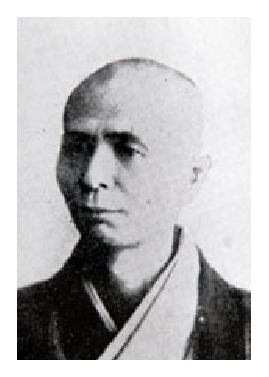
\includegraphics[width=0.25\textwidth]{Shuei.eps}
\caption*{\label{fig:Shuei}Honinbo Shuei}
\end{wrapfigure}

Part of the strength of Honinbo Shuei was his flexibility in \textit{joseki}: though neither a promoter of excessive influential or territorial play, he was happy to modify how he played in the corner to the demands of the position at hand. His games are a rich source especially of \textit{tenuki} \textit{joseki}, in which he ignores a position one, twice, or sometimes even three times whilst his opponent plays there; and then returns. His most lasting gift to the game, though was his invention of the 3-3 invasion under a 4-4, which he passed on to his pupil Tamura Yasuhisa (later Honinbo Shusai) and which came to popularity in the \textit{shin fuseki} era. \\

\section*{Go Seigen (1914 – 2014)}

\begin{wrapfigure}{L}{0.3\textwidth}
\centering
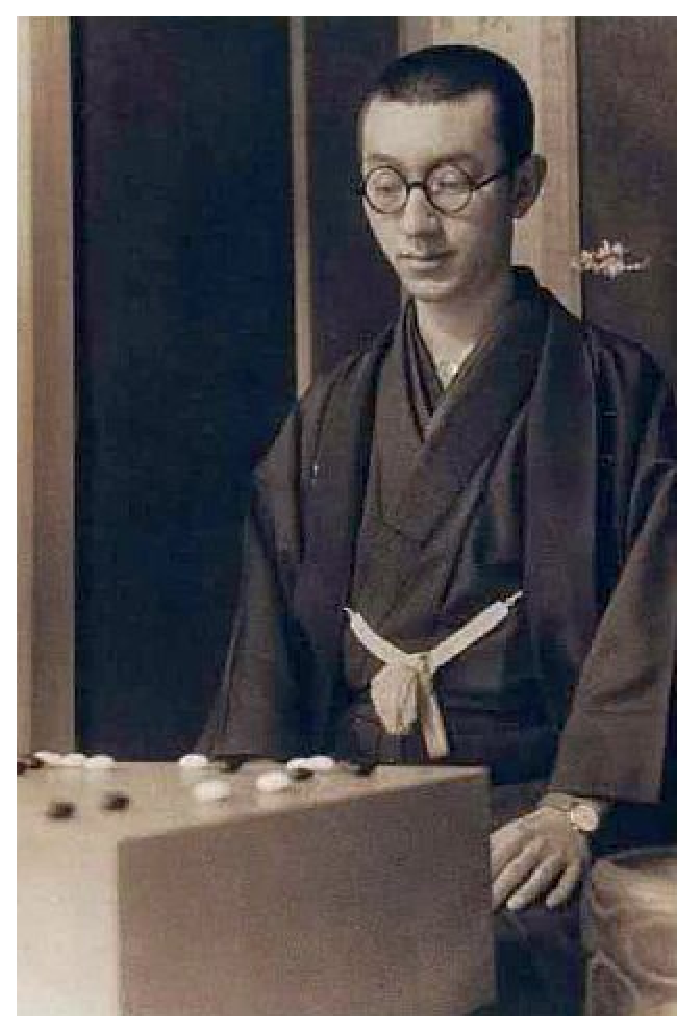
\includegraphics[width=0.25\textwidth]{GoSeigen.eps}
\caption*{\label{fig:Seigen}Go Seigen}
\end{wrapfigure}

Go Seigen was his Japanese name. In China he was known as Wu Quan and later Wu Qingyuan.\\

Go Seigen often innovated in \textit{joseki} to gain what he judged to be a better result than provided by the sequences of the time, or perhaps sometimes just to lure his opponent `out of book' where he could overpower them with superior reading. One invention of his is particularly well known: a major discovery in the large avalanche \textit{joseki}, a complex sequence which is mentioned briefly in the 3-4 section of this book.\todo{Which diagram? to cross-reference}\\

\clearpage

\section*{Kitani Minoru (1909 – 1975)}

\begin{wrapfigure}{L}{0.3\textwidth}
\centering
\includegraphics[width=0.25\textwidth]{kitani.eps}
\caption*{\label{fig:Kitani}Kitani Minoru}
\end{wrapfigure}

Kitani Minoru was possibly the most prolific innovator of the 20th century in simple \textit{joseki}. He developed a swathe of basic \textit{joseki} to suit his periods of territorial style; often, these were avoided by most other professionals as they were considered to neglect the issue of influence too much in their focus on point-taking. However, it should not be forgotten that Kitani was also a major innovator of influential \textit{joseki}: in fact he was the very first professional to play the 5-5 point, and developed a range of sequences in which it was used.\\

\section*{AlphaGo (developed in 2015)}

\begin{wrapfigure}{R}{0.3\textwidth}
\centering

\includegraphics[width=0.25\textwidth]{AlphaGo.eps}
\caption*{\label{fig:AlphaGo}AlphaGo}
\end{wrapfigure}

AlphaGo is profoundly different from the other players on this list – it is not a human but a highly sophisticated computer program. Each version of AlphaGo was characteristically different in how it approached the game: it began with a human-like style, then later began to value influence highly, but eventually settled on a highly territorial strategy. AlphaGo has taken its hand to the potter's wheel of \textit{joseki} creation on many occasions, sometimes producing surprising results, but its greatest impact has been on the theory of 3-3 point invasion beneath a 4-4. It values the 3-3 point highly, plays it early and often, and has produced a whole new toolset of sequences which modern players are still eagerly exploring.\\

\end{document}
